\section{Physics objects} \label{sec:objects}

\graphicspath{{3_DataAnalysisStrategy/Figures}}

A global event reconstruction using the Particle Flow (PF) algorithm \cite{cms:particle_flow} is carried out in order to
identify each particle in the 
event\footnote{An event typically refers to a single proton-proton bunch crossing, occuring
every $25$ nanoseconds at the LHC.}. 
PF algorithm accomplishes this by combining detector hit information
from all different sub-detectors within CMS. The specific information used to determine the energy
and momentum of a particle depends on the identity of the particle: Whether it is a photon, muon, electron,
neutral hadron or charged hadron. Photons are identified as ECAL energy clusters that are not linked to 
any charged particle tracks (following from the fact that they are electrically neutral). 
Electrons are identified as a primary charged particle track, potentially 
together with ECAL energy clusters that are consistent with either the extrapolation of this track or possible
bremsstrahlung photons emitted when the electron passes through the tracker material. Muons are identified as 
consistent charged particle tracks in both the central tracker and the muon system, as well as potential energy
clusters in the calorimeters that are consistent with the tracks. Tracks that are not already assigned to electrons or muons,
together with calorimeter energy deposits, are identified as charged hadrons. Finally, neutral hadrons are identified using leftover 
HCAL and ECAL clusters after the identification of charged hadrons. A schematic summarizing the particle identification in CMS
is shown in Fig.~\ref{fig:particle_detection_cms}.

\begin{figure}[htbp]
    \centering
    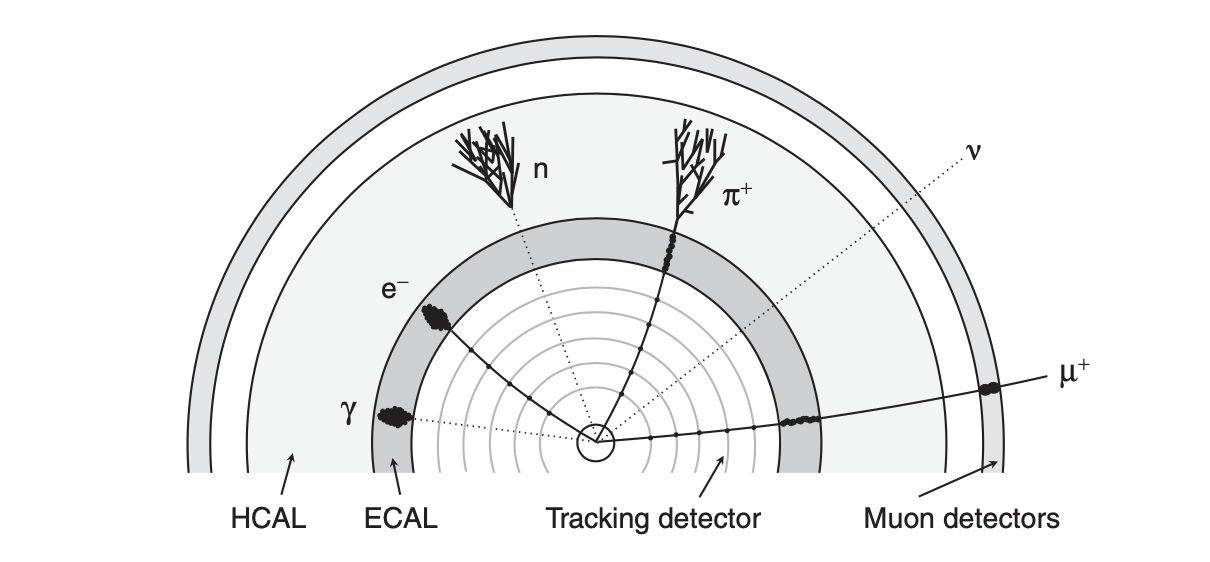
\includegraphics[width=0.7\textwidth]{particle_detection_schematic.png}
    \caption{A schematic representing the particle detection at the CMS detector.
    Hadrons (e.g. $n$, $\pi^{\pm}$) are detected as hadronic showers of particles (jets)
    due to color confinement, and weakly interacting particles such as neutrinos ($\nu$) pass through the
    detector without interaction. Schematic is taken from~\cite{Thomson:2013zua}.}
    \label{fig:particle_detection_cms}
\end{figure}

Since a bunch of protons are collided during each bunch crossing, multiple collision vertices arise
due to multiple interactions within the bunch. Aim of the event reconstruction is to select a primary
collision vertex, which is determined as the vertex containing the largest sum of squared transverse momenta,
$p_{T}^2$, from associated tracks \cite{cms:phase2_upgrade}.
Tracks and energy content from the rest of the vertices are very commonly referred as pileup (PU). Thanks to the assignment of the
primary vertex, charged particles can be filtered out from the main event if their tracks are found to be originating 
from a non-primary vertex. This allows to reduce the PU contribution in the reconstructed event. 

In the following subsections, details of how different physics objects are reconstructed will be discussed. To aid the
discussion, signal region (SR) refers to the set of selections used to collect VBF $\hinv$ signal events,
and control regions (CR) refer to the set of selections used to measure and constrain the dominant background yields
in the signal region.

\subsection{Jets}
\label{sec:objects_jets}

A typical jet consists of a shower of hadrons generated by a single quark or gluon.
In this analysis, jets are reconstructed by clustering reconstructed particles
using the anti-$k_{T}$ algorithm~\cite{Cacciari:2008gp}. Jets are
clustered with a distance parameter of $R = 0.4$ and are referred to as AK4
jets. Prior to clustering, charged particles whose tracks are found to be associated
with a non-primary vertex is removed to reduce the energy contributions from other
vertices. This technique is referred to as ``Charged Hadron Subtraction (CHS)''~\cite{CMS:2014ata}. 

Jet momentum is determined as the vector sum of all particle momenta
in the jet, and is found from simulation to be within 5 to 10\% of the
true momentum over the full $p_{T}$ spectrum and detector acceptance. 
A set of jet energy corrections are applied to correct the jet momenta for various effects,
and bring the reconstructed jet energy to the simulated jet energy ratio closer to $1$.
First, jet energies are further corrected for PU effects, mostly coming from neutral 
particles in the jet after the application of CHS, by using an event-by-event energy density estimation
to derive an offset energy to subtract from the jet energy.
After this, jet momenta are further corrected by using corrections derived from events
where a jet recoils against a well-identified object, including $Z(\ell\ell)\;+$ jet and
$\gamma\;+$ jet events~\cite{Khachatryan:2016kdb}. 
For the analysis that will be explained in this thesis, the
\texttt{Summer19UL17\_V5} and \texttt{Summer19UL18\_V5} versions of
the jet energy corrections are used for the 2017 and 2018 datasets,
respectively~\cite{JME:JECRecommendations}. On top of the jet energy corrections,
jet energy resolution (JER) corrections are also applied to correct for differences of 
jet resolution between data and simulation.

The AK4 jets used in this analysis are required to pass the 
loose identification criteria \cite{CMS:JME_jetId}, and AK4 jets with $p_{T} < 50$ GeV 
must pass the pileup identification (ID) criteria \cite{CMS:JME_jetPuID}. 
Pileup ID criteria aims to reduce the contribution from
pileup by removing jets from the event which contain a large amount of energy from secondary vertices
within the bunch crossing.

% In addition to the pileup ID requirement, jet energy resolution (JER) corrections are applied to all AK4 jets. 
% Application of this correction on all jets is observed to improve the jet modeling, especially at the region near $|\eta| = 2.9$. 
% The effect of JER corrections is shown in Fig.~\ref{fig:jer_correction}, where the $\eta$ distribution is plotted
% for the second-highest $p_{T}$ (subleading) jet in the event, with and without the JER corrections applied.

% \begin{figure}[htb]
%     \begin{minipage}[t]{\linewidth}\centering
%         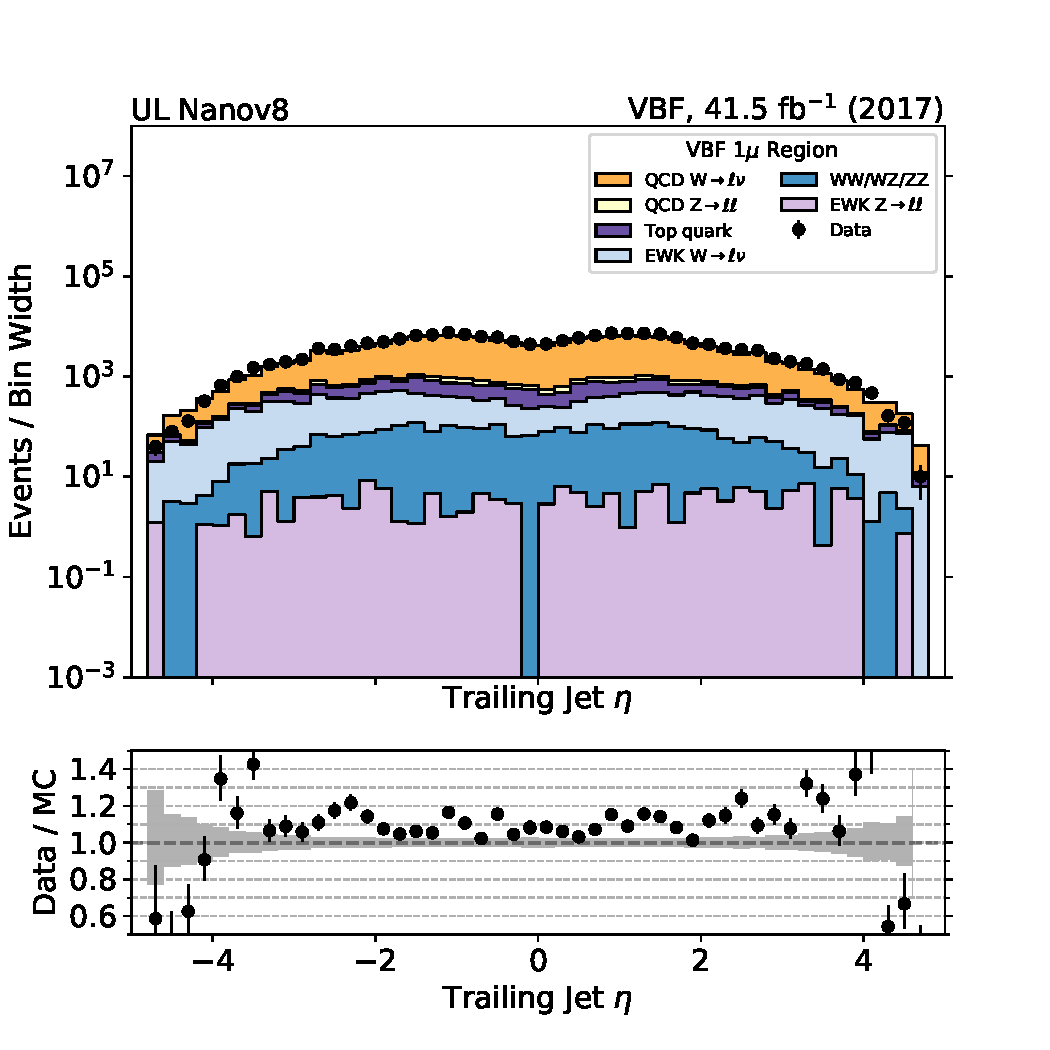
\includegraphics[width=0.45\textwidth]{DataMC/JERImpact/cr_1m_vbf_data_mc_ak4_eta1_2017_withJER.pdf}
%         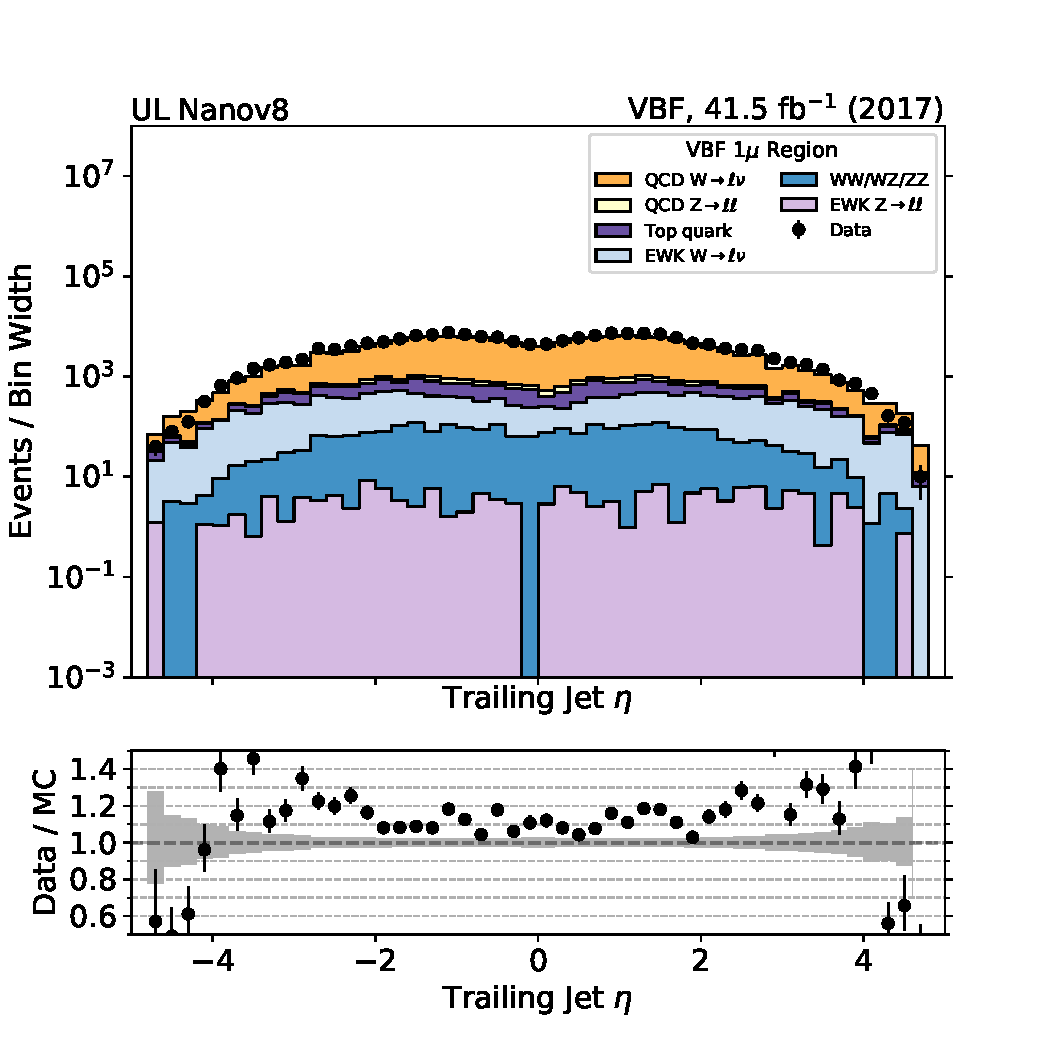
\includegraphics[width=0.45\textwidth]{DataMC/JERImpact/cr_1m_vbf_data_mc_ak4_eta1_2017_noJER.pdf}
%     \end{minipage}
%     \caption{Subleading AK4 jet $\eta$ distribution in single muon control region with JER corrections applied (left) 
%     and without JER corrections applied (right).}
%     \label{fig:jer_correction}
% \end{figure}

In addition, jet-lepton overlap cleaning is done by removing any AK4 jet that is within a cone of radius
$\Delta R = \sqrt{\Delta \eta^2 + \Delta \phi^2} = 0.4$ surrounding a lepton or a photon. Only lepton and 
photon candidates satisfying the object criteria described below are considered during the cleaning.
Lastly, if the leading or the subleading jet is found to be within the tracker coverage (i.e. $|\eta| < 2.5$),
constraints on the charged hadron and neutral hadron energy fractions of the jet ($R_{CHEF}$, $R_{NHEF}$ respectively) 
are placed such that $R_{CHEF} > 0.1$ and 
$R_{NHEF} < 0.8$. If a jet is found to violate these requirements, it is removed from the event.
These additional requirements aid in rejecting mis-identified jets with spuriously low charged hadron 
fractions\footnote{On average, one would expect $\approx 60\%$ of jet energy to be in the form of charged particles
(e.g. from charged pions $\pi^{\pm}$). Hence a reconstructed jet with $<10 \%$ charged energy fraction is highly unexpected and potentially 
due to mis-identification of other particles or detector noise.}.

\subsubsection{b-tagged jets}
\label{subsec:objects_bjets}

Identifying jets that originate from a b-quark is important in this analysis, since a b-quark is not expected in the
final state of the VBF $H \rightarrow inv.$ signal (for example, see Fig.~\ref{fig:vbfhinv_signal_diag}), 
and vetoing events with b-jets in the final state allows to remove most of the 
backgrounds originating from top quark production.

In this analysis, jets with $p_{T} > 20$ GeV and $|\eta| < 2.4$ are identified as b-jets according to the
DeepCSV algorithm\footnote{Lifetime of hadrons containing b-quarks are
relatively large, $\tau \sim 1.5$ ps, giving rise to a few milimetres of displacement from the primary vertex
before further decay, hence creating a second, displaced vertex. b-tagging algorithms like DeepCSV make use of
this feature to classify a jet as coming from a b-quark or not.}~\cite{Sirunyan:2017ezt}. 
A medium working point is adopted, corresponding to correctly identifying a b-jet with a
probability of 80\%, and mis-identifying a light-flavor jet with a probability of 10\%. This working point corresponds to the value of 
DeepCSV tagger to be greater than 0.4506 in 2017, and 0.4168 in 2018.

\subsection{Missing transverse momentum and recoil}
\label{subsec:objects_met_recoil}

The vector \ptvecmiss is defined as the imbalance in the transverse
momentum of all particles that interact with the detectors.
Due to momentum conservation in the plane transverse to the beam axis, \ptvecmiss
corresponds to the transverse momentum that is carried by undetected particles such as neutrinos.
Large $\ptvecmiss$ can also imply the observation of a $\hinv$ signal, due to the decay products
of the Higgs boson passing undetected through the detector\footnote{Further discussion
on this can be found in the Introduction chapter, please see Sec.~\ref{subsec:exp_signatures}.}.
Therefore, $\ptvecmiss$ is a key variable in this analysis.   
It is computed as the negative of the vectorial sum of transverse
momenta of all Particle Flow (PF) candidates and is therefore also referred to as PF \ptvecmiss.
The magnitude of the \ptvecmiss is referred to as \ptmiss.

Minimum energy thresholds in the calorimeters, inefficiencies
in the tracker, nonlinearity of the response of the calorimeter
for hadronic particles can lead to an over- or underestimation of \ptmiss.
The bias on the \ptmiss measurement is reduced by propagating the effect of the jet energy
corrections introduced in Sec.~\ref{sec:objects_jets} according to

\begin{equation}
\ptvecmiss(\mathrm{corr})
=\ptvecmiss - \sum_\mathrm{jets} (\vec{p}_\mathrm{T,jet}({\mathrm{corr}})-\vec{p}_\mathrm{T,jet}),
\label{eq:Type1MET}
\end{equation}
where the ``corr'' refers to the energy corrected measurements
of the related objects.
This correction for \ptvecmiss uses jet energy scale corrections
for all corrected jets with $\pt > 15$ GeV that have less than $90 \%$
of their energy deposited in the ECAL. Furthermore, if a muon is found in a
jet, its 4-momentum is subtracted from the 4-momentum of the jet
when performing the correction and is added back to a corrected object.

Since VBF \hinv signal events in this analysis contain only jets and no other 
reconstructed visible candidates in the final state,
\ptmiss is equivalent to the total hadronic momentum in the event that is transverse to the proton-proton collision axis. 
For the leading $Z(\nu\nu)$ + jets and $W(\ell\nu)$ + jets backgrounds which can result in the same final state 
(described in Sec.~\ref{subsec:sr_vbf_selection}), 
$\ptmiss$ corresponds to the transverse momentum of the $Z$ and $W$ boson, respectively. 
To mimic this behavior in in the control regions of this analysis, the hadronic recoil
$\vec{U}$ is used, which is defined as the sum of the transverse
momenta of all particles except the vector boson (or its decay products).
The hadronic recoil $\vec{U}$ is computed as

\begin{equation}
  \vec{U} = \ptvecmiss + \sum _{i\;\in\;\textrm{leptons, photons}}\ptveci
  \label{eq:recoil_def}
\end{equation}

where the sum takes into account the leptons and photons used to define the respective control 
region\footnote{Please see Sec.~\ref{sec:event_selection} for the discussion of all control regions
used in the analysis.}.
As an example, in the control region where $\Zmmjets$ events are collected, the recoil $\vec{U}$ can be
computed as $\vec{U} = \ptvecmiss + \sum_{i\;\in\;\textrm{muons}} \ptveci$, where the sum goes over
the two reconstructed muons, which are the decay products of the $Z$ boson. Here, assumming small $\ptvecmiss$
due to the fact that the final state muons will not result in transverse momentum imbalance, 
$\vec{U} \approx \sum_{i\;\in\;\textrm{muons}} \ptveci \approx \vec{p}_T^{\;Z}$. Hence,
in all regions in the analysis, $\vec{U}$ can be thought of as the transverse momentum of the $Z$, $W$ or $\gamma$ 
boson, depending on the control region being considered.
For the signal region, 
since there are no reconstructed leptons in the final state, it should be noted that the sum term
in Eq.~\ref{eq:recoil_def} will be $0$, hence making $\vec{U} = \ptvecmiss$ for the signal 
region\footnote{But still, please note that $\vec{U} \approx \vec{p}_T^{\;V}$ condition holds true in the
signal region for $\Vjets$ backgrounds, where $V = Z, W$. Hence the definition of hadronic recoil $\vec{U}$ is consistent
across all regions in the analysis.}.

% The uncertainty of \ptmiss has a strong dependence on the
% event topology. Therefore, the uncertainty on \ptmiss is often factorized into its components of
% jets, leptons and unclustered energy. Each sub-component is then varied
% within its scale and resolution uncertainty.

In addition to the events with genuine $\ptmiss$, such as $Z(\nu\nu)$ + jets, 
anomalous high-\ptmiss events can also appear due to various phenomena.
In the ECAL, spurious deposits may appear due to particles striking
sensors in the ECAL photodetectors, or from real showers with non-collision
origins such as those caused by beam halo particles. ECAL dead cells can cause real
energy to be missed, again leading to a spurious imbalance.
In the HCAL, spurious energy can arise due to  noise in the hybrid
photodiode and readout box  electronics, as well as
direct particle interactions with  the light guides and
photomultiplier tubes of the forward calorimeter. 
A number of filters has been developed by the POG/DPG groups to identify and suppress anomalous high
\ptmiss events~\cite{CMS-JME-TWIKI-FILTER}. The recommended filters are listed in Tab.~\ref{tab:metfilters} and are applied in the analysis.

\begin{table}[ht!]
    \centering
    \small
    \def\arraystretch{1.5}
    \caption{The \ptmiss filters recommended by the JME POG~\cite{CMS-JME-TWIKI-FILTER}. 
    The recommendations apply to both 2017 and 2018. Except for the bad super cluster filter (``EE badSC''), all filters are applied both in data and simulation (MC).}
    \begin{tabular}{p{5cm} p{7cm} p{2cm} }
        \hline
        \hline
                                           &                                                                     \\
        Filter                             & Name in input dataset                    & Applied in data (MC)     \\\hline
        Primary vertex filter              & Flag\_goodVertices                       & \checkmark  (\checkmark) \\
        Beam halo filter                   & Flag\_globalSuperTightHalo2016Filter     & \checkmark  (\checkmark) \\
        HBHE noise filter                  & Flag\_HBHENoiseFilter                    & \checkmark  (\checkmark) \\
        HBHEiso noise filter               & Flag\_HBHENoiseIsoFilter                 & \checkmark  (\checkmark) \\
        ECAL TP filter                     & Flag\_EcalDeadCellTriggerPrimitiveFilter & \checkmark  (\checkmark) \\
        Bad PF Muon Filter                 & Flag\_BadPFMuonFilter                    & \checkmark  (\checkmark) \\
        EE badSC noise filter              & Flag\_eeBadScFilter                      & \checkmark  ($\times$)     \\
        ECAL bad calibration filter update & Flag\_ecalBadCalibFilter               & \checkmark  (\checkmark) \\
        \hline
    \end{tabular}

    \label{tab:metfilters}
\end{table}

\subsection{Leptons}

\subsubsection{Muons}
\label{subsec:muons}

Muons are reconstructed by combining information from silicon tracker detector and the muon detection system
\cite{cms:muon_paper}. Requirements for a good-quality muon object include the fit quality of the
muon track, and its consistency with the primary vertex in the event. All muons considered in this
analysis have $p_T > 10$ GeV and $|\eta| < 2.4$ (i.e. they are reconstructed within the tracker range).

Two types of muon identification are used for this analysis, which are termed as loose and tight muons \cite{CMS-MUO-TWIKI-IDLOOSE,CMS-MUO-TWIKI-IDTIGHT}.
Loose muon identification is used to identify muons in the signal region and veto them\footnote{This selection is due to the fact that
final state muons are not expected in VBF $\hinv$ signal events. As explained later in Sec.~\ref{subsec:sr_vbf_selection}, this veto
helps suppressing background processes such as $\Wmnjets$ and $\Zmmjets$.}. 
Tight muon identification, on the other hand,
has more strict quality conditions and are used to identify good quality muons in $W(\mu \nu)$ and $Z(\mu \mu)$ control regions.

Loose muon objects must pass the following requirements \cite{CMS-MUO-TWIKI-IDLOOSE}:

\begin{itemize}
    \item It must be reconstructed as a muon by the Particle Flow (PF) algorithm
    \item Must have $p_T > 10$ GeV and $|\eta| < 2.4$
\end{itemize}

Tight muons pass all the requirements of loose muons, together with passing these additional muon quality requirements \cite{CMS-MUO-TWIKI-IDTIGHT}:

\begin{itemize}
    \item Must have $p_T > 20$ GeV and $|\eta| < 2.4$
    \item Normalized $\chi^2$ of the muon track fit $<$ 10
    \item At least one Muon Chamber hit must be included in the muon track fit
    \item Muon segments required in at least two muon stations
    \item The muon track must have transverse impact parameter $d_{xy} < $ 2~mm w.r.t. the primary vertex
    \item The longitudinal distance of the tracker track w.r.t. the primary vertex must be $d_z < $ 5~mm
    \item Number of pixel hits $>$ 0
    \item Cut on number of tracker layers with hits $>$ 5
\end{itemize}

In addition to the requirements listed above, an energy isolation requirement is imposed on the muons. An isolation variable 
is computed based on the sum of energies of nearby PF candidates, within $\Delta R < 0.4$ of the muon. This isolation
variable is then used to select muons that are relatively isolated from other physical objects. This isolation variable
is required to be less than $0.25$ for loose muons, and less than $0.15$ for tight muons.


\subsubsection{Electrons}
\label{subsec:electrons}

Electrons are reconstructed using the information from the tracker and the ECAL detector \cite{cms:elepho_paper}. All electrons
considered in this analysis have $p_T > 10$ GeV and $|\eta| < 2.5$.

Similar to the case of muons, two types of identification are used for electrons, which are labeled as veto and tight electrons.
Veto electrons are used to identify electrons in the signal region and veto events containing such 
electrons\footnote{Similar to the case of muons, such a veto helps suppressing background processes such as
$\Wevjets$ and $\Zeejets$ in the signal region.}. 
Tight electrons, which have tighter
quality cuts, are used to identify electrons in $W(e \nu)$ and $Z(ee)$ control regions.

The quality requrements for veto and tight electron objects are different for electrons reconstructed in the barrel region
($|\eta| < 1.479$) and in the endcap region ($|\eta| > 1.479$). The details of the quality requirements are listed in Tables \ref{tab:veto_electron_def_barrel},
\ref{tab:tight_electron_def_barrel}, \ref{tab:veto_electron_def_endcap} and \ref{tab:tight_electron_def_endcap}.

\begin{table}[htbp]
\centering
\def\arraystretch{1.2}

\begin{tabular}{|l|c|}
    \hline\hline
    Quantity & Requirement \\\hline
    Full 5x5 $\sigma_{i\eta i\eta}$ &  $< 0.0126$ \\
    $|\Delta\eta_{\mathrm{seed}}|$ & $< 0.00463$  \\
    $|\Delta\phi_{\mathrm{In}}|$ & $< 0.148$ \\
    H/E & $<$ 0.05+1.16/$E_{\mathrm{SC}}$+0.0324$\rho$/$E_{\mathrm{SC}}$ \\
    Relative Isolation With EA & $<$ 0.198+0.506/$p_T$ \\
    $|$1/E-1/p$|$ & $< 0.209$ \\
    Expected Missing Inner Hits & $\leq$ 2 \\
    Pass conversion veto & yes \\
    \hline\hline
\end{tabular}
\caption{Requirements used to define veto electrons in the barrel region ($|\eta| < 1.479$).}
\label{tab:veto_electron_def_barrel}
\end{table}

\begin{table}[htbp]
\centering
\def\arraystretch{1.2}
\begin{tabular}{|l|c|}
    \hline\hline
    Quantity & Requirement \\\hline
    Full 5x5 $\sigma_{i\eta i\eta}$ &  $< 0.0104$ \\
    $|\Delta\eta_{\mathrm{seed}}|$ & $< 0.00255$  \\
    $|\Delta\phi_{\mathrm{In}}|$ & $< 0.022$ \\
    H/E & $<$ 0.026+1.15/$E_{\mathrm{SC}}$+0.0324$\rho$/$E_{\mathrm{SC}}$ \\
    Relative Isolation With EA & $<$ 0.0287+0.506/$p_T$ \\
    $|$1/E-1/p$|$ & $< 0.159$ \\
    Expected Missing Inner Hits & $\leq$ 1 \\
    Pass conversion veto & yes \\
    \hline\hline
\end{tabular}
\caption{Requirements used to define tight electrons in the barrel region ($|\eta| < 1.479$).}
\label{tab:tight_electron_def_barrel}
\end{table}

\begin{table}[htbp]
\centering
\def\arraystretch{1.2}
\begin{tabular}{|l|c|}
    \hline\hline
    Quantity & Requirement \\\hline
    Full 5x5 $\sigma_{i\eta i\eta}$ &  $< 0.0457$ \\
    $|\Delta\eta_{\mathrm{seed}}|$ & $< 0.00814$  \\
    $|\Delta\phi_{\mathrm{In}}|$ & $< 0.19$ \\
    H/E & $<$ 0.05+2.54/$E_{SC}$+0.183$\rho$/$E_{SC}$ \\
    Relative Isolation With EA & $<$ 0.203+0.963/$p_T$ \\
    $|$1/E-1/p$|$ & $< 0.132$ \\
    Expected Missing Inner Hits & $\leq$ 3 \\
    Pass conversion veto & yes \\
    \hline\hline
\end{tabular}
\caption{Requirements used to define veto electrons in the endcap region ($|\eta| > 1.479$).}
\label{tab:veto_electron_def_endcap}
\end{table}

\begin{table}[htbp]
\centering
\def\arraystretch{1.2}
\begin{tabular}{|l|c|}
    \hline\hline
    Quantity & Requirement \\\hline
    Full 5x5 $\sigma_{i\eta i\eta}$ &  $< 0.0353$ \\
    $|\Delta\eta_{\mathrm{seed}}|$ & $< 0.00501$  \\
    $|\Delta\phi_{\mathrm{In}}|$ & $< 0.0236$ \\
    H/E & $<$ 0.0188+2.06/$E_{SC}$+0.183$\rho$/$E_{SC}$ \\
    Relative Isolation With EA & $<$ 0.0445+0.963/$p_T$ \\
    $|$1/E-1/p$|$ & $< 0.0197$ \\
    Expected Missing Inner Hits & $\leq$ 1 \\
    Pass conversion veto & yes \\
    \hline\hline
\end{tabular}
\caption{Requirements used to define tight electrons in the endcap region ($|\eta| > 1.479$).}
\label{tab:tight_electron_def_endcap}
\end{table}

In addition to the requirements listed in the tables above, electrons are cross-cleaned against the muons
within $\Delta R < 0.3$.

\subsubsection{Taus}

Hadronically decaying $\tau$ leptons are required to pass identification criteria
using the DeepTau algorithm~\cite{CMS-DP-2019-033}. In addition, $\tau$ candidates are required to be isolated from other activity in the
event. The isolation requirement is computed by summing the \pt of the charged PF
candidates and PF photon candidates within an isolation cone of $\Delta R = 0.5$,
around the tau candidate direction. 
% The other charged lepton candidates and photon candidates associated with the
% tau candidate are removed from this sum and further described in Ref.~\cite{Khachatryan:2015dfa}.
The ``VVLoose'' isolation working point~\cite{taupog_twiki} is employed in this analysis
for tau candidates with $\pt > 20$ GeV within $|\eta| < 2.3$. $\tau$ candidates within $\Delta R = 0.4$ of 
an identified veto electron or loose muon are rejected. If hadronically decaying taus are reconstructed within
an event that satisfy the conditions mentioned above, the event is rejected from the analysis to suppress 
backgrounds coming from the hadronic decays of tau leptons. 

\subsection{Photons}
\label{subsec:photons}

Photon candidates are reconstructed from energy deposits in the ECAL using algorithms
that constrain the clusters to the size and shape expected from a photon~\cite{CMS:EGM-14-001}.
The identification of the candidates is based on shower-shape and isolation variables.
For isolated photons, scalar sums of the \pt of PF candidates within a cone of $\Delta R < 0.3$
around the photon candidate are required to be below the bounds defined. Only the PF candidates
that do not overlap with the electromagnetic shower of the candidate photon are included in the isolation sums.

Similar to electrons and muons, two candidate definitions are employed for photons. Loose photons are used to reject
events with reconstructed photons in the signal region. These photons are required to pass the EGamma POG loose identification criteria~\cite{CMS-EGM-TWIKI-GAMID},
have $\pt > 15$ GeV and be within $|\eta|<2.5$. The exact identification criteria for loose photons in barrel and endcap 
are summarized in Tables.~\ref{tab:PhotonIDLooseBarrel} and~\ref{tab:PhotonIDLooseEndcap}, respectively.
Tight photons are used to identify photon objects in the dedicated photon control region. 
These photons are explicitly required to be in the barrel ($|\eta|<1.479$), and have $\pt>230$ GeV. The identification criteria for tight photons
are summarized in Table~\ref{tab:PhotonIDTight}.

\begin{table}[htb!]
    \centering
    \small
    \def\arraystretch{1.2}
    \begin{tabular}{l c}
    \hline
    Variable                                   &  Selection       \\
                                               &  Barrel ($|\eta|<1.479$) \\
    \hline
    \hline
    Full 5x5 $\sigma_{i\eta i\eta}$            & $< 0.0106 $    \\
    H/E                                        & $<  0.04596 $    \\
    charged hadron isolation                   & $< 1.694 $     \\
    neutral hadron isolation                   & $< 24.032 + 0.01512\times p_T+2.259\times 10^{-5} \times {p_T}^2$ \\
    photon isolation                           & $< 2.876 + 0.004017\times p_T$  \\
    Conversion safe electron veto              & Yes           \\
    \hline
    \end{tabular}
    \caption{Loose photon identification criteria for photons in the barrel. These photons must also have $\pt > 15$ GeV.}
    \label{tab:PhotonIDLooseBarrel}
\end{table}

\begin{table}[htb!]
    \centering
    \small
    \def\arraystretch{1.2}
    \begin{tabular}{l c}
    \hline
    Variable                                   &  Selection       \\
                                               &  Endcap ($1.479<|\eta|<2.5$)  \\
    \hline
    \hline
    Full 5x5 $\sigma_{i\eta i\eta}$            & $< 0.0272 $    \\
    H/E                                        & $< 0.0590 $    \\
    charged hadron isolation                   & $< 2.089 $     \\
    neutral hadron isolation                   & $< 19.722 + 0.0117\times p_T+2.3\times 10^{-5} \times {p_T}^2$ \\
    photon isolation                           & $< 4.162 + 0.0037\times p_T$  \\
    Conversion safe electron veto              & Yes           \\
    \hline
    \end{tabular}
    \caption{Loose photon identification criteria for photons in the endcap. These photons must also have $\pt > 15$ GeV.}
    \label{tab:PhotonIDLooseEndcap}
\end{table}

\begin{table}[htb!]
    \centering
    \small
    \def\arraystretch{1.2}
    \begin{tabular}{l c}
    \hline
    Variable                                   &  Selection       \\
                                               &  Barrel  \\
    \hline
    \hline
    Full 5x5 $\sigma_{i\eta i\eta}$            & $<  0.01015  $ \\
    H/E                                        & $<  0.02197  $   \\
    charged hadron isolation                   & $< 1.141  $     \\
    neutral hadron isolation                   & $< 1.189  + 0.01512\times p_T+2.259\times 10^{-5} \times {p_T}^2$ \\
    photon isolation                           & $< 2.08 + 0.004017\times p_T$  \\
    Conversion safe electron veto              & Yes           \\
    \hline
    \end{tabular}
    \caption{Tight photon identification criteria. The criteria are only given for the barrel region since endcap photons are not 
    considered in the analysis.}
    \label{tab:PhotonIDTight}
\end{table}

\subsubsection{Photon purity}
\label{subsec:photonpurity}

Photons are reconstructed from ECAL clusters, and can be discriminated from other sources of ECAL deposits due 
to the properties of the cluster, as well as their lack of other associated signatures such as tracks or HCAL 
deposits. This discrimination is not perfect, however, and in some cases, non-photon objects will incorrectly be 
identified as photons, which in this text are also referred to as ``fake photons''.
The leading source of fake photons is QCD production of multijet events, where 
a jet is misidentified as a photon. The QCD process is relevant mainly because of its large cross-section, which yields non-negligible 
contributions to the photon selection even if the per-jet probability of misreconstruction is small.

To estimate the fake contribution to the photon control region, a purity measurement is performed. The photon purity is 
defined as the fraction of reconstructed photons that is actually due to an isolated photon from the hard scattering event, 
as opposed to a fake. The purity is obtained from a template fit to the distribution of the \sieie variable in data, where 
\sieie variable represents the width of the ECAL shower in the $\eta$ direction. Due to the different shower behavior of 
photons and hadrons, the \sieie distribution shows characteristically different behavior between these two classes of 
reconstructed photons: Real photons show a large peak with a cut-off at around $\sieie\approx0.01$, while fake photons will 
have a smaller peak (stemming from actual photons inside jets), and an additional non-peaking bulk region at larger 
\sieie (stemming from hadrons interacting in the ECAL). The inputs to the fit are defined as follows:

\begin{itemize}
\item Photons in data are selected by applying the same identification criteria as for the tight selection defined above, 
with the exception of the \sieie requirement. By removing this requirement, the full \sieie distribution can be observed.

\item A real photon template is obtained from $\gamma +$ jets Monte Carlo (MC) simulation. The same identification criteria are applied as in data.

\item A fake photon template is obtained from data. In this case, the identification criteria are modified by requiring that 
at least one of the isolation criteria is not passed. Therefore, the photons in this template represent reconstructed photons inside jets,
(i.e. ``fake photons").

\end{itemize}

The templates are derived in separate bins of the photon $\pt$ and the measurement is performed separately for 2017 and 2018. 
Events are selected using the following criteria:

\begin{itemize}
    \item At least one jet with $\pt>100$ GeV and $|\eta|<2.4$, which is not overlapping with a photon of interest.
    \item The event must pass the \texttt{HLT\_Photon200} trigger, which requires a photon with $\pt > 200$ GeV to be reconstructed at the HLT level.
    \item The event must pass the offline MET filters, and have $\ptmiss < 60$ GeV.
\end{itemize}

The fits are shown in Figs.~\ref{fig:purity_fits_2017} and~\ref{fig:purity_fits_2018}. The resulting impurity values as a function of photon \pt 
are shown in Fig.~\ref{fig:purity_result}. While the fits are performed in the range of $0.04<\sieie<0.15$, the purity is evaluated only taking 
into account the contributions with $\sieie<0.01$, which is the requirement posed in the identification criteria used in the analysis (see Tab.~\ref{tab:PhotonIDTight}).  
Overall, good fit performance is observed and the impurity is found to range between $1\%$ and $4\%$, with a decreasing trend with increasing photon \pt. 
Residual differences between the best fit and the data appear because the template shapes do not match the data shapes perfectly. To take this 
effect into account, the measurement is repeated with four alternative binning schemes that range from being very fine to very coarse and are shown in 
Fig.~\ref{fig:purity_binning}. By varying the binning choice, the effect of shape differences can be amplified or mitigated, and its impact on the 
final impurity values can be tested. The spread of the resulting values per bin is found to be small and a 25\% uncertainty is assigned to the impurity 
and thus the QCD background estimate. For application in the analysis, the nominal impurity values are interpolated using an exponential function fit.

\begin{figure}[htbp]
    \centering
        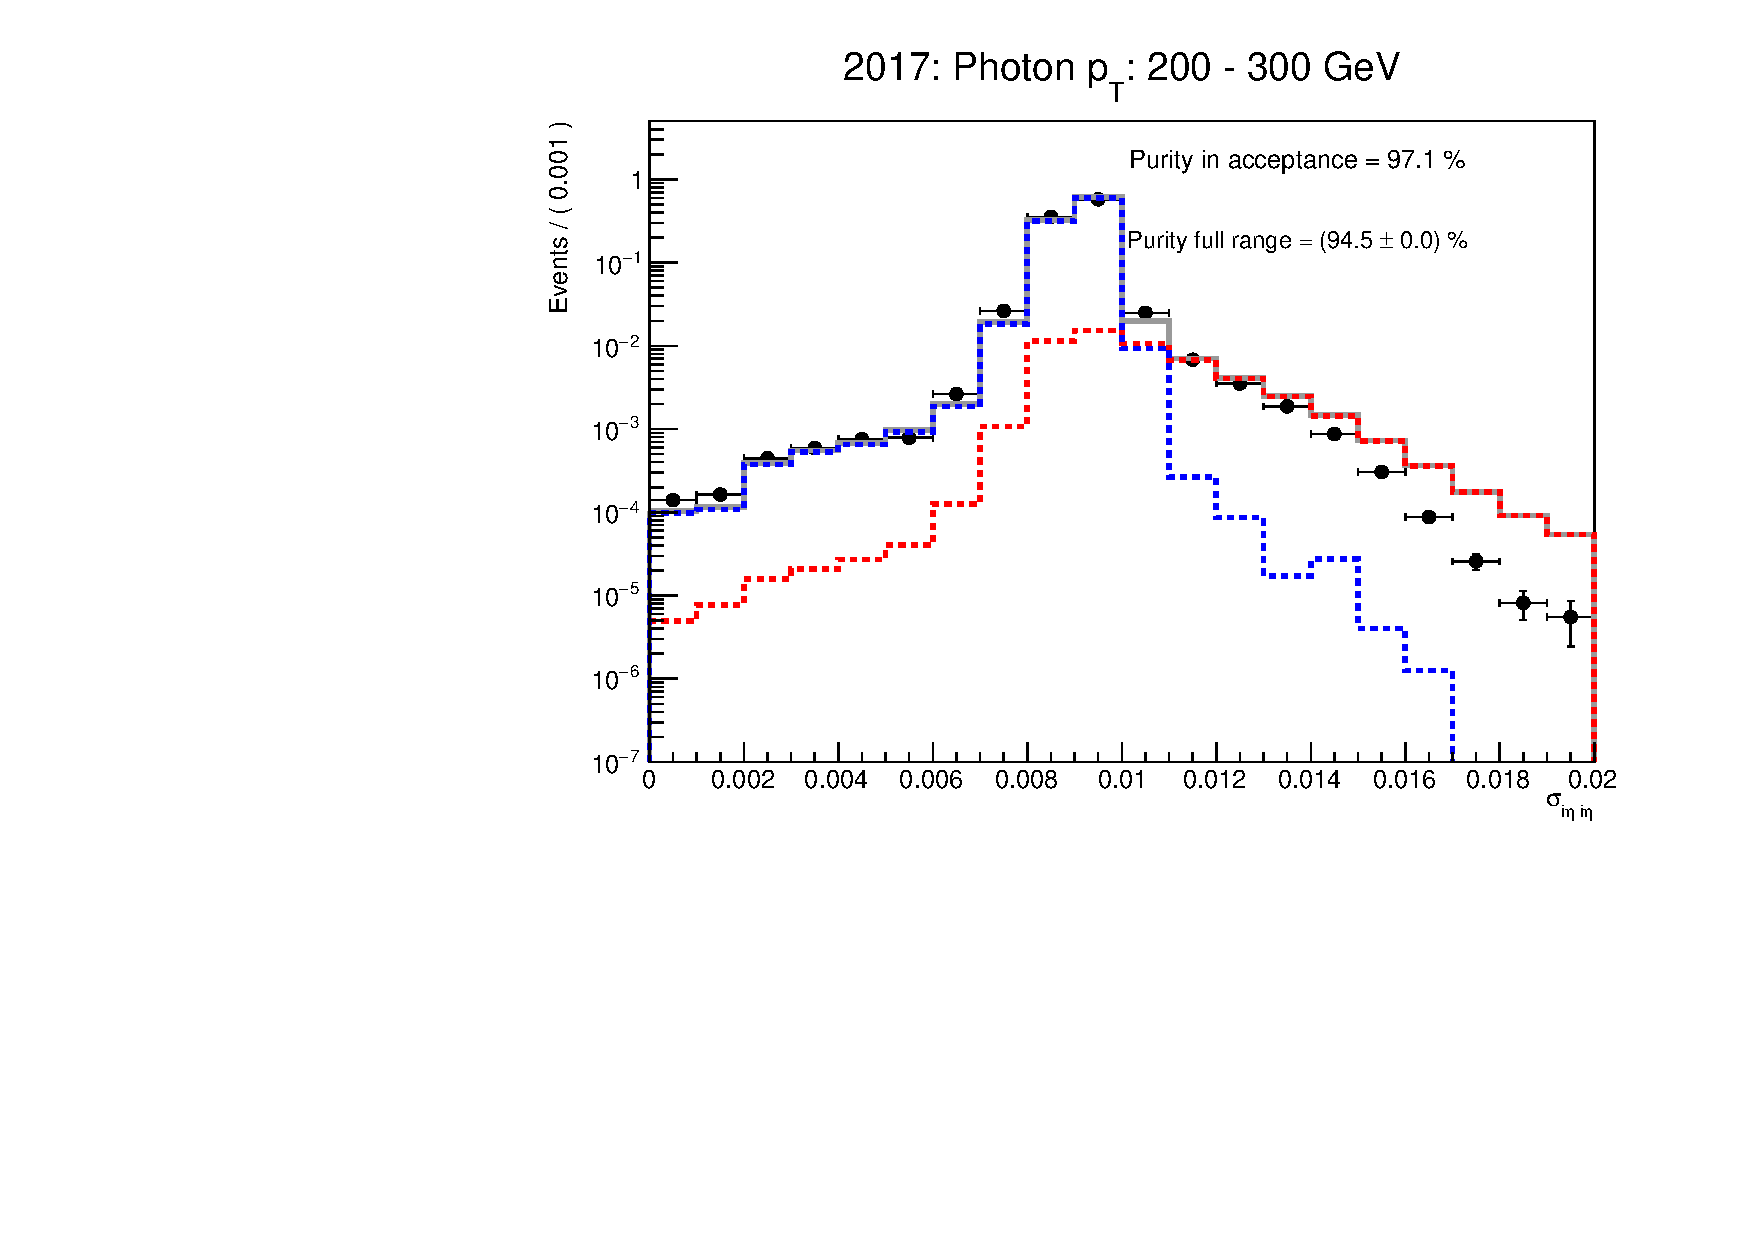
\includegraphics[width=0.45\textwidth]{PhotonPurity/fit_2017_pt200-300_nominal.pdf}
        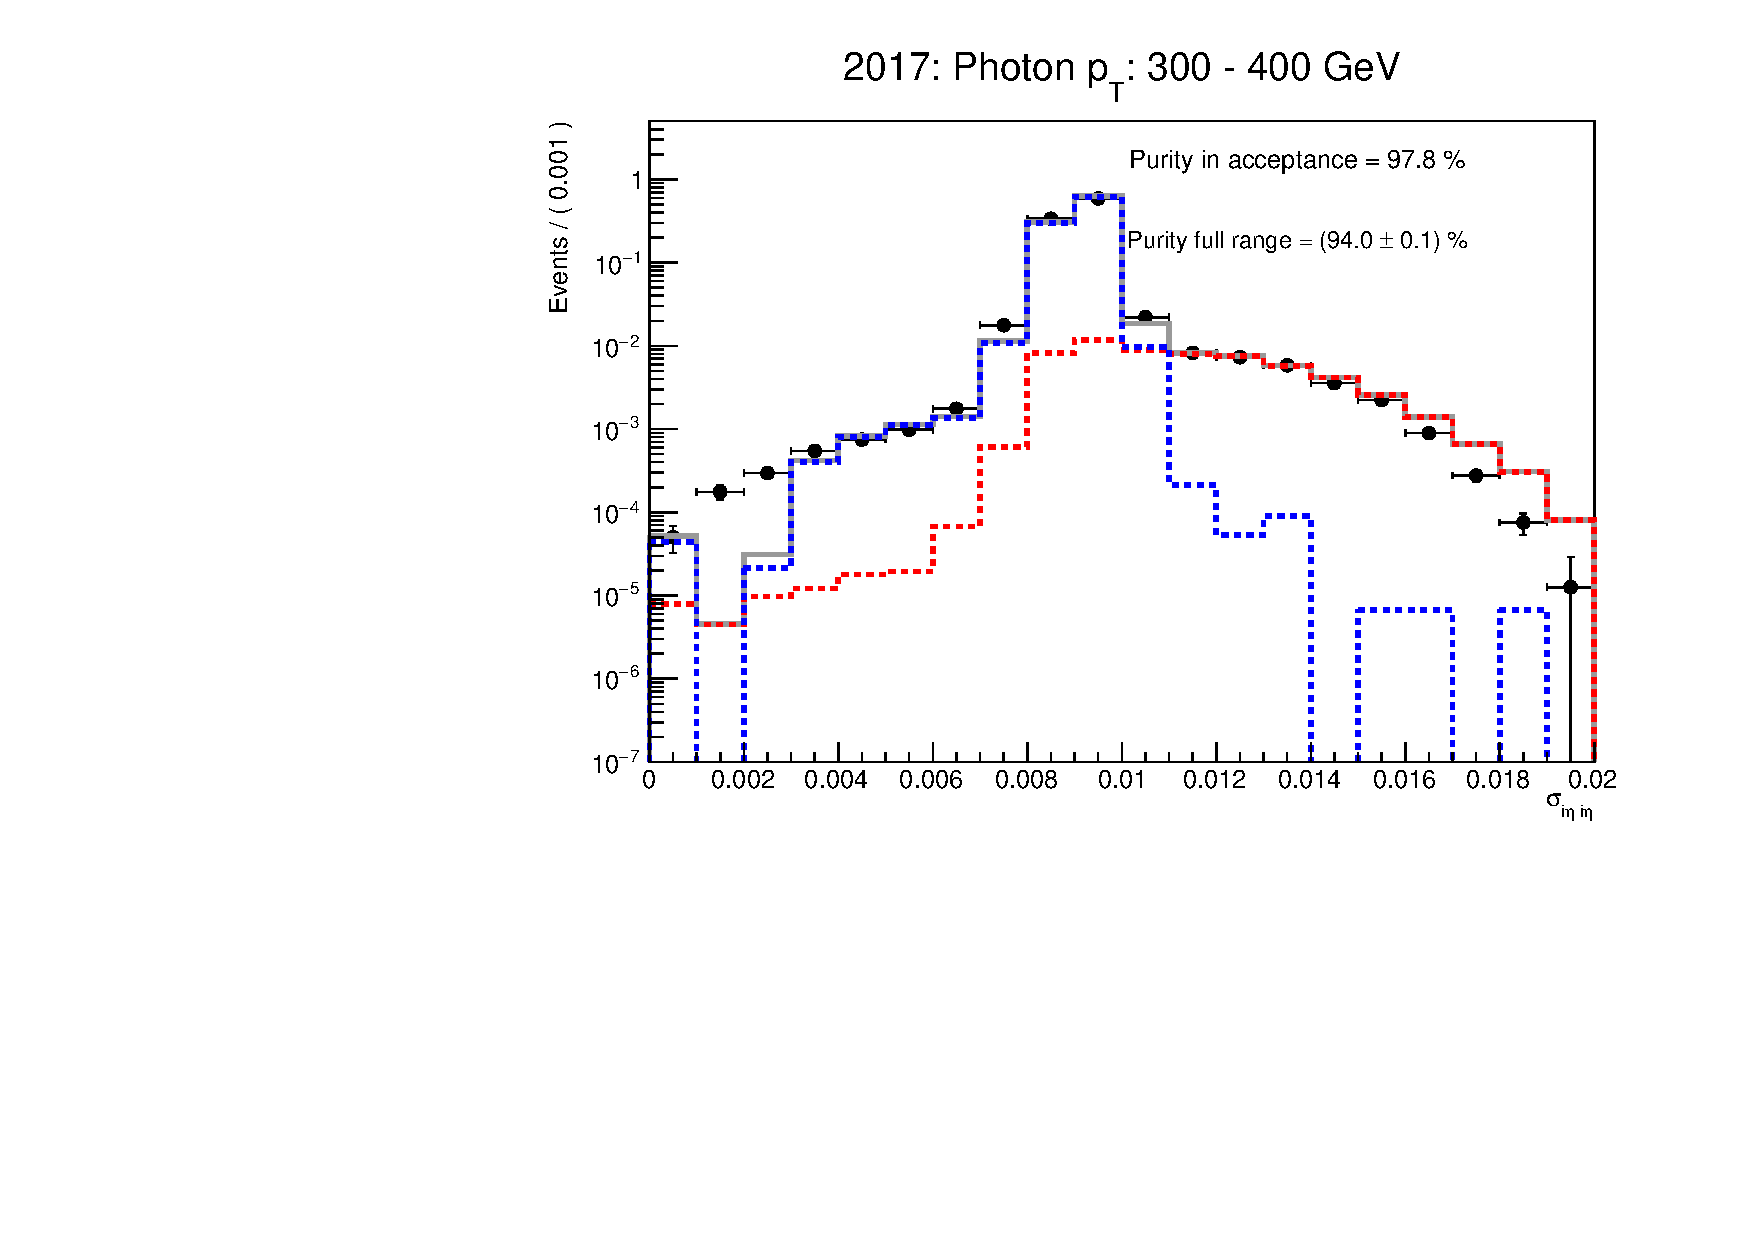
\includegraphics[width=0.45\textwidth]{PhotonPurity/fit_2017_pt300-400_nominal.pdf}
        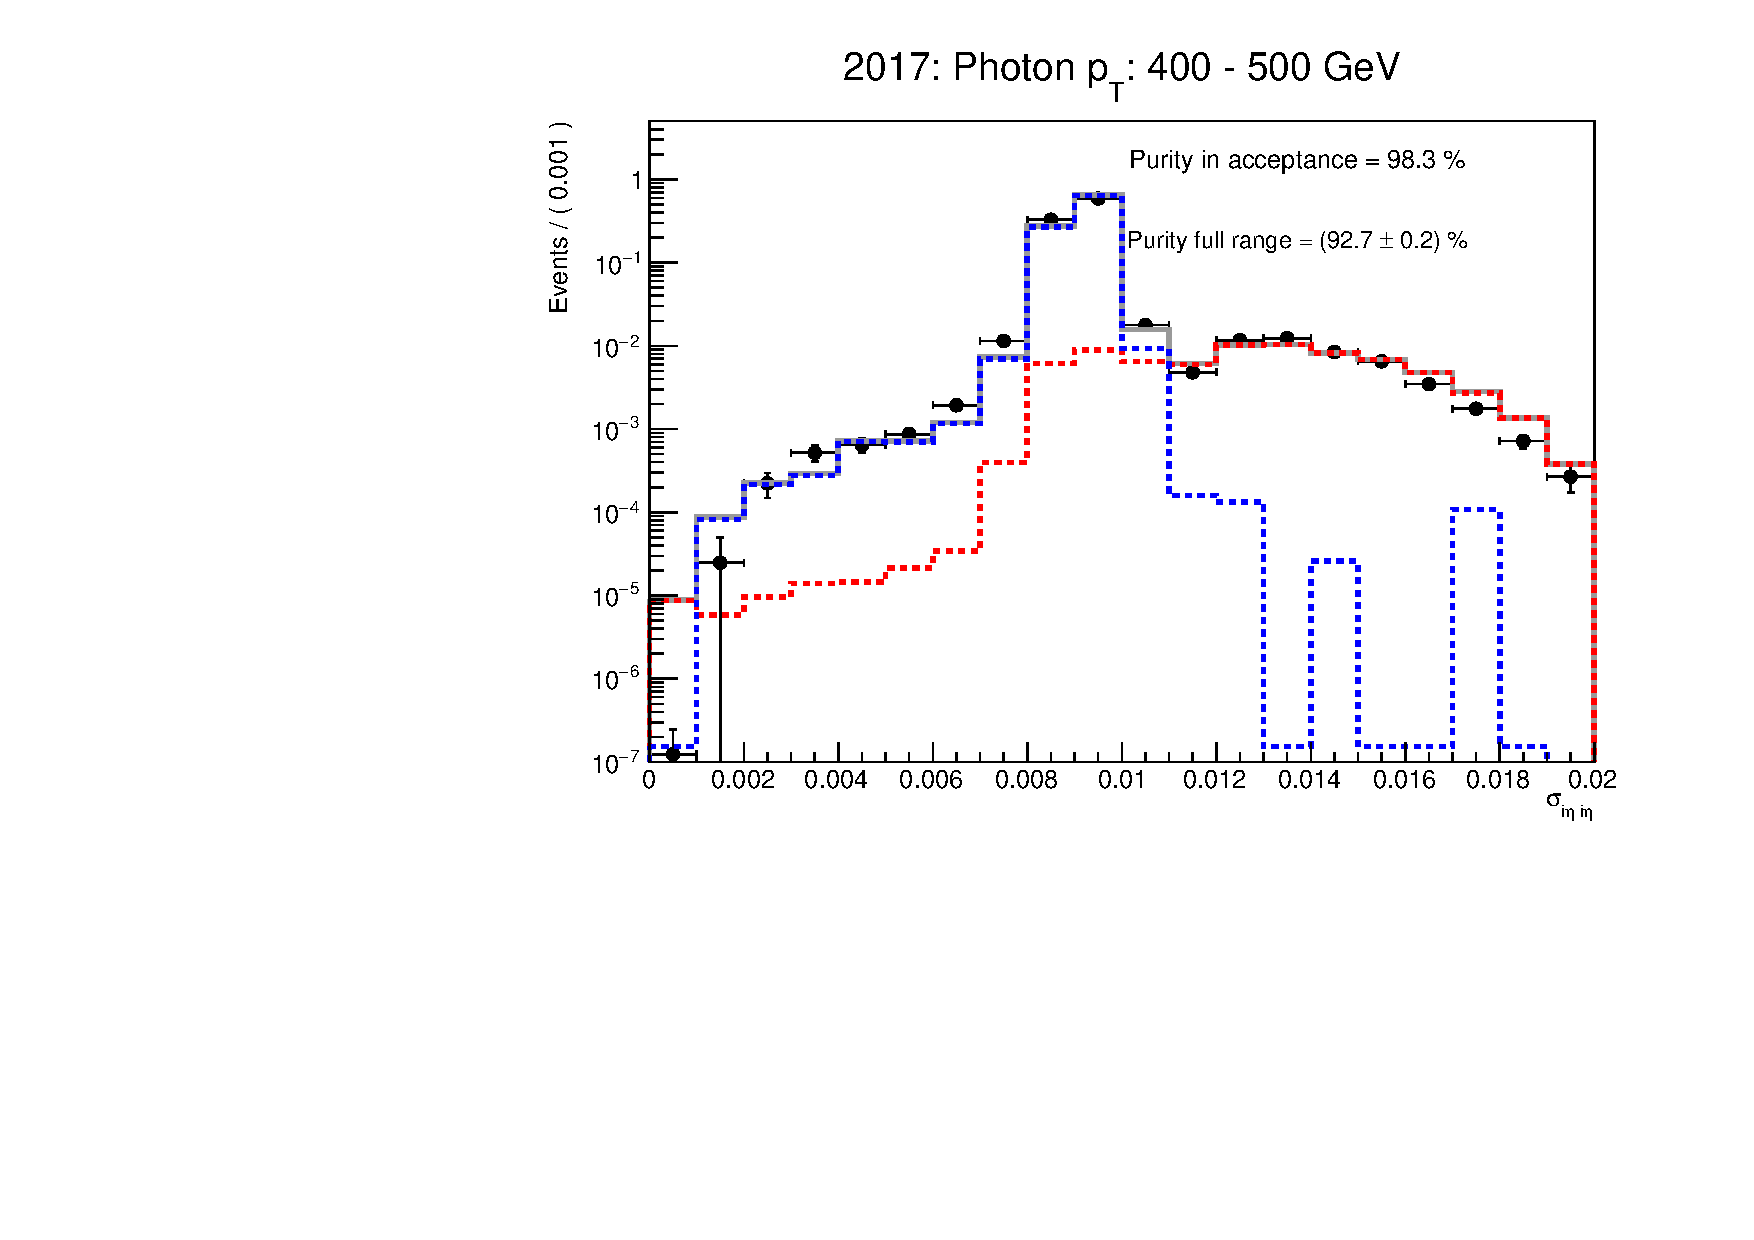
\includegraphics[width=0.45\textwidth]{PhotonPurity/fit_2017_pt400-500_nominal.pdf}
        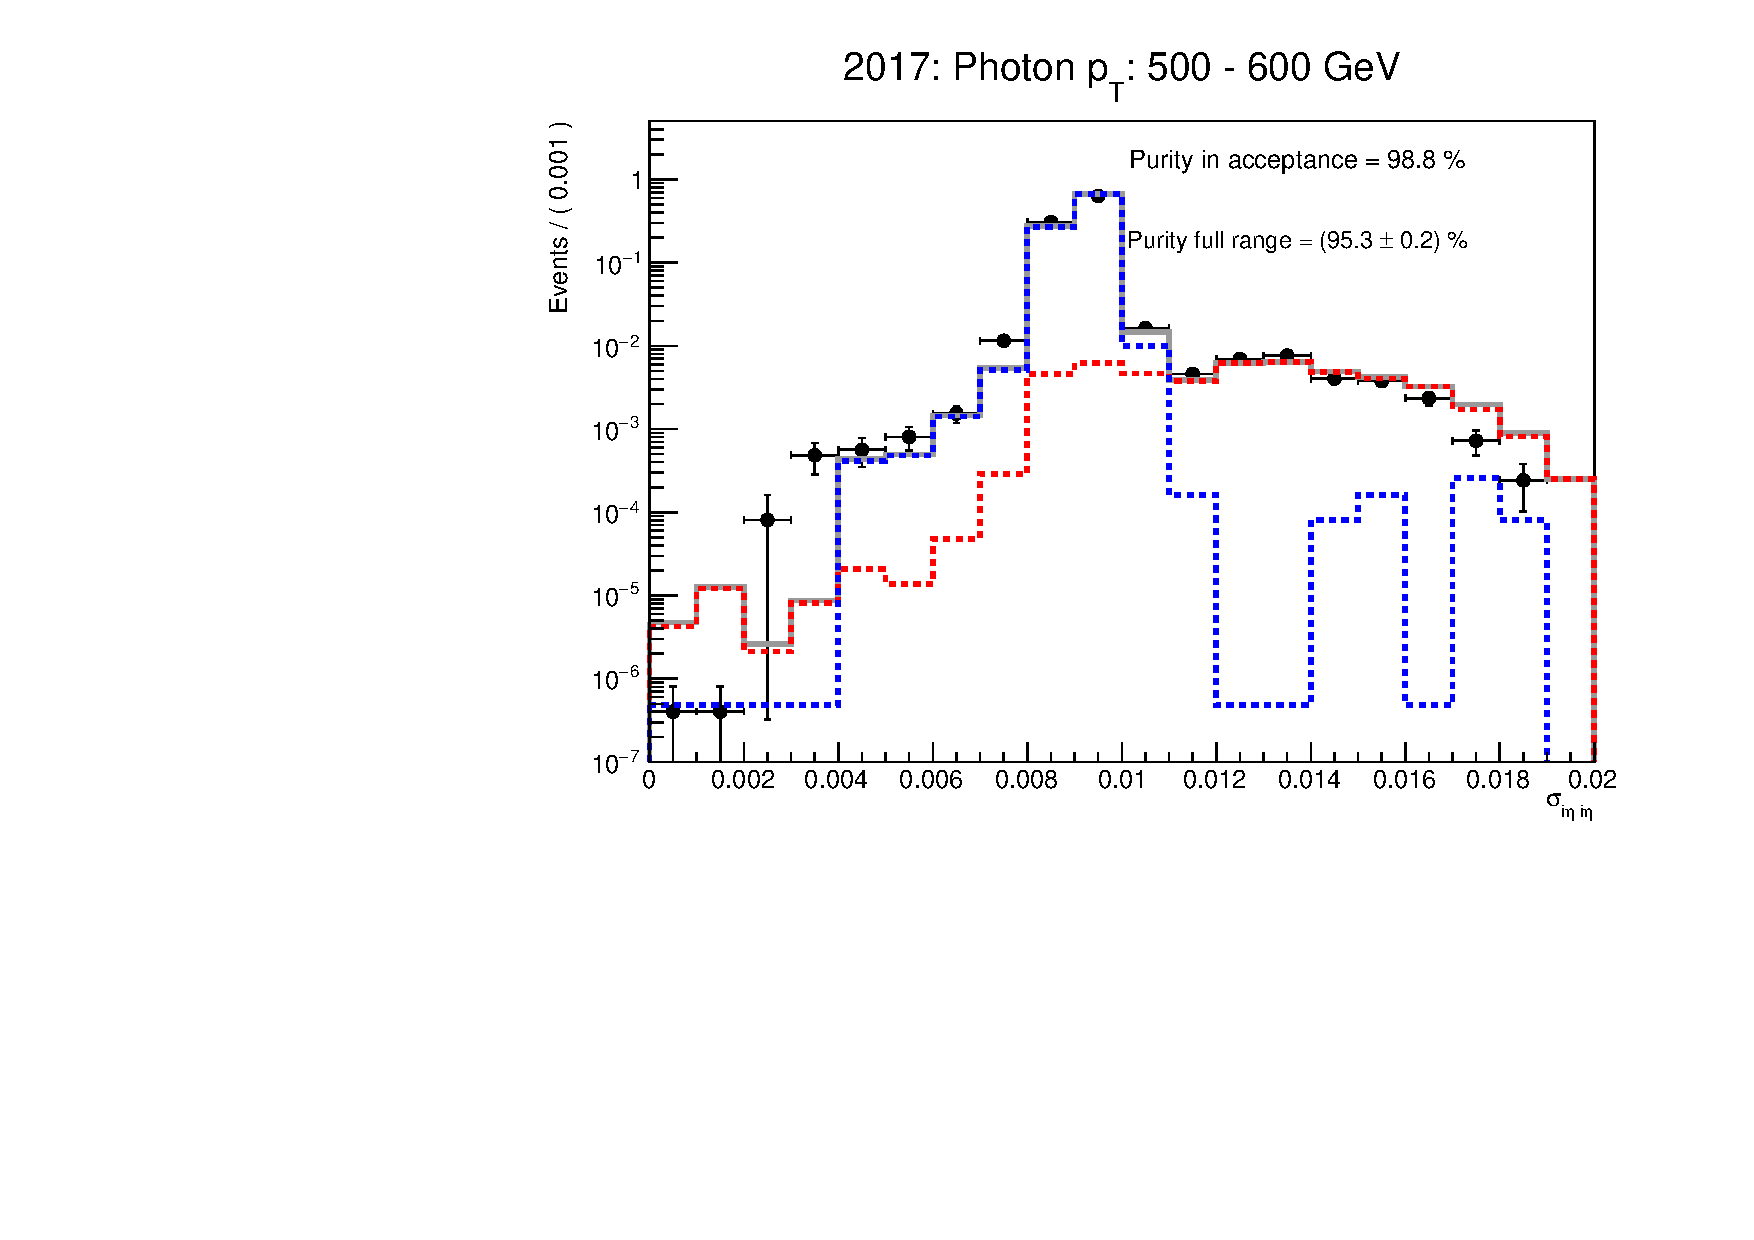
\includegraphics[width=0.45\textwidth]{PhotonPurity/fit_2017_pt500-600_nominal.pdf}
        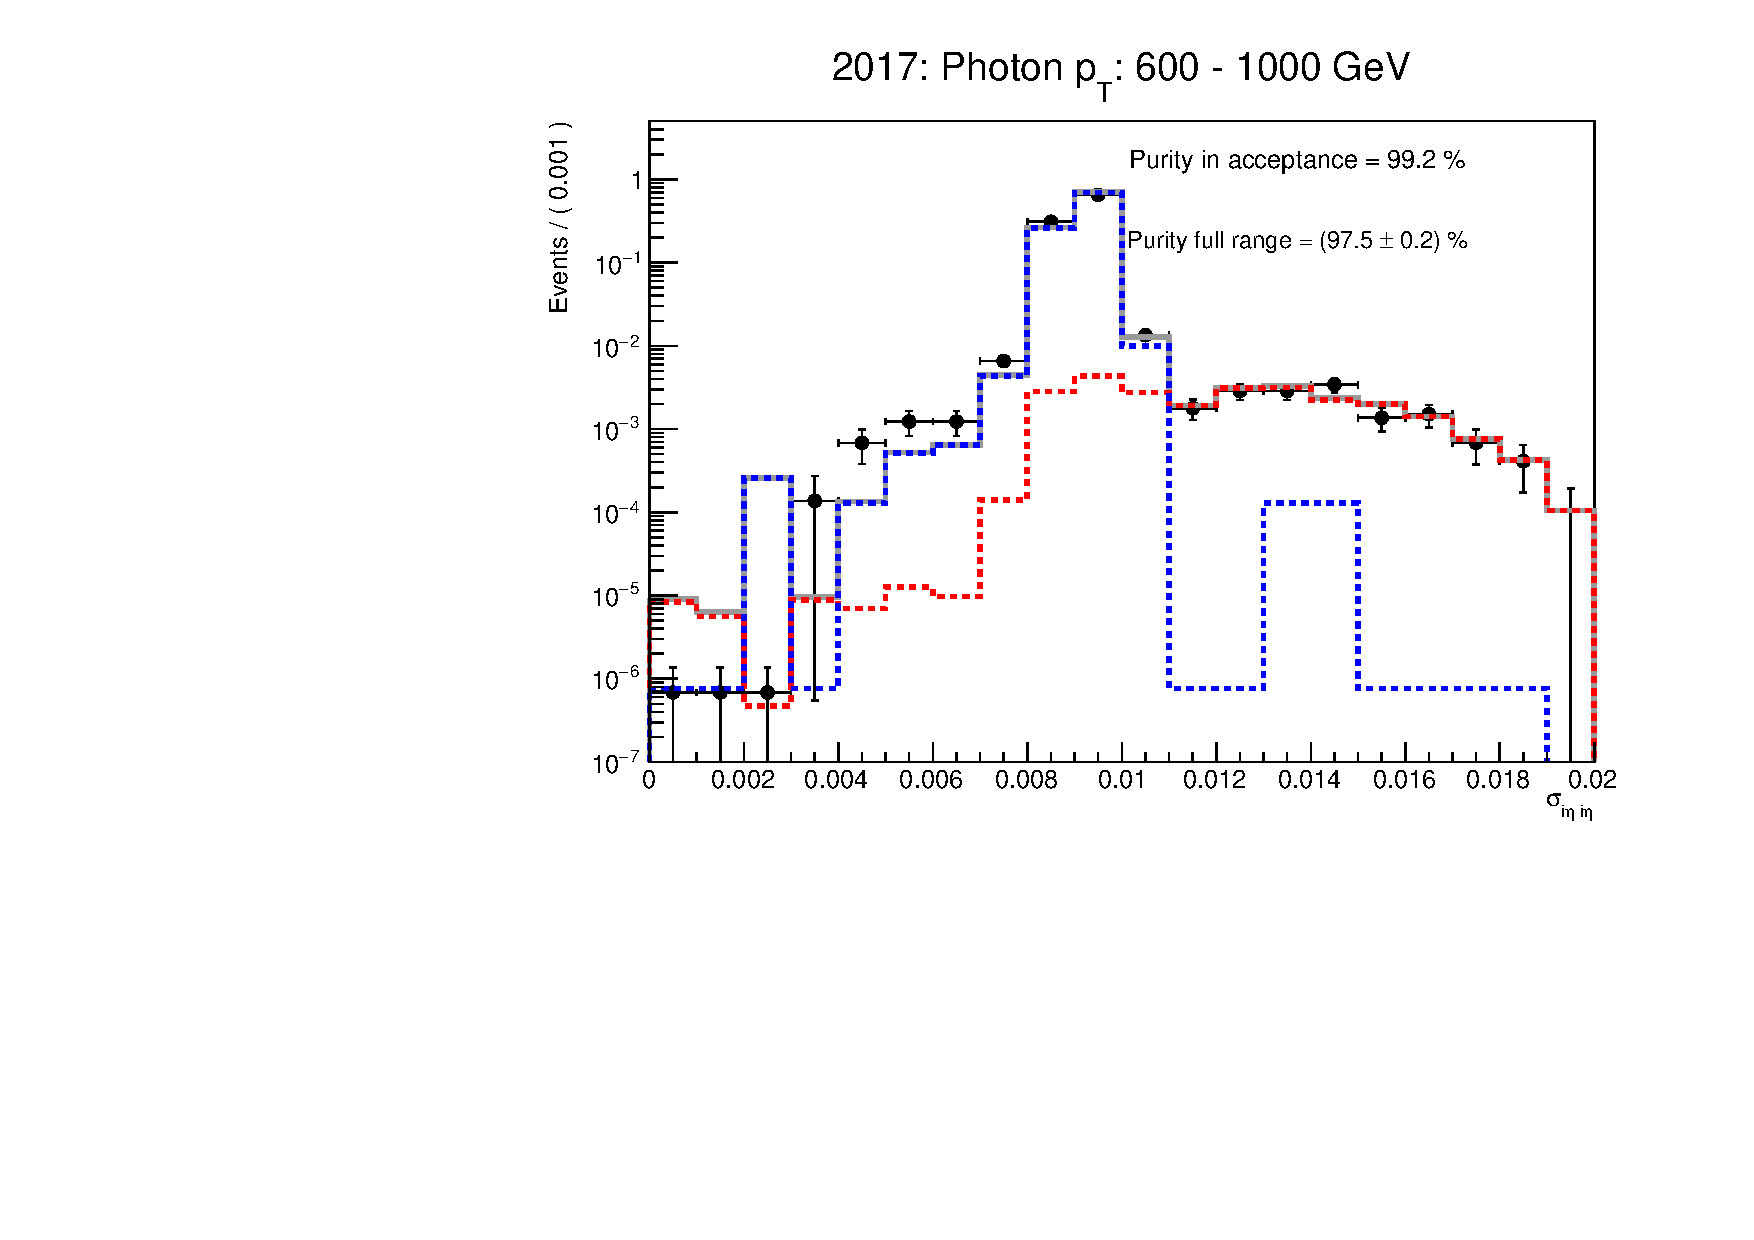
\includegraphics[width=0.45\textwidth]{PhotonPurity/fit_2017_pt600-1000_nominal.pdf}
    \caption{Template fits used to determine the photon purity in the 2017 dataset. The fits are shown in bins of photon \pt, increasing from left 
    to right and top to bottom. The ``nominal'' binning scheme is used.}
    \label{fig:purity_fits_2017}
\end{figure}

\begin{figure}[htbp]
    \centering
        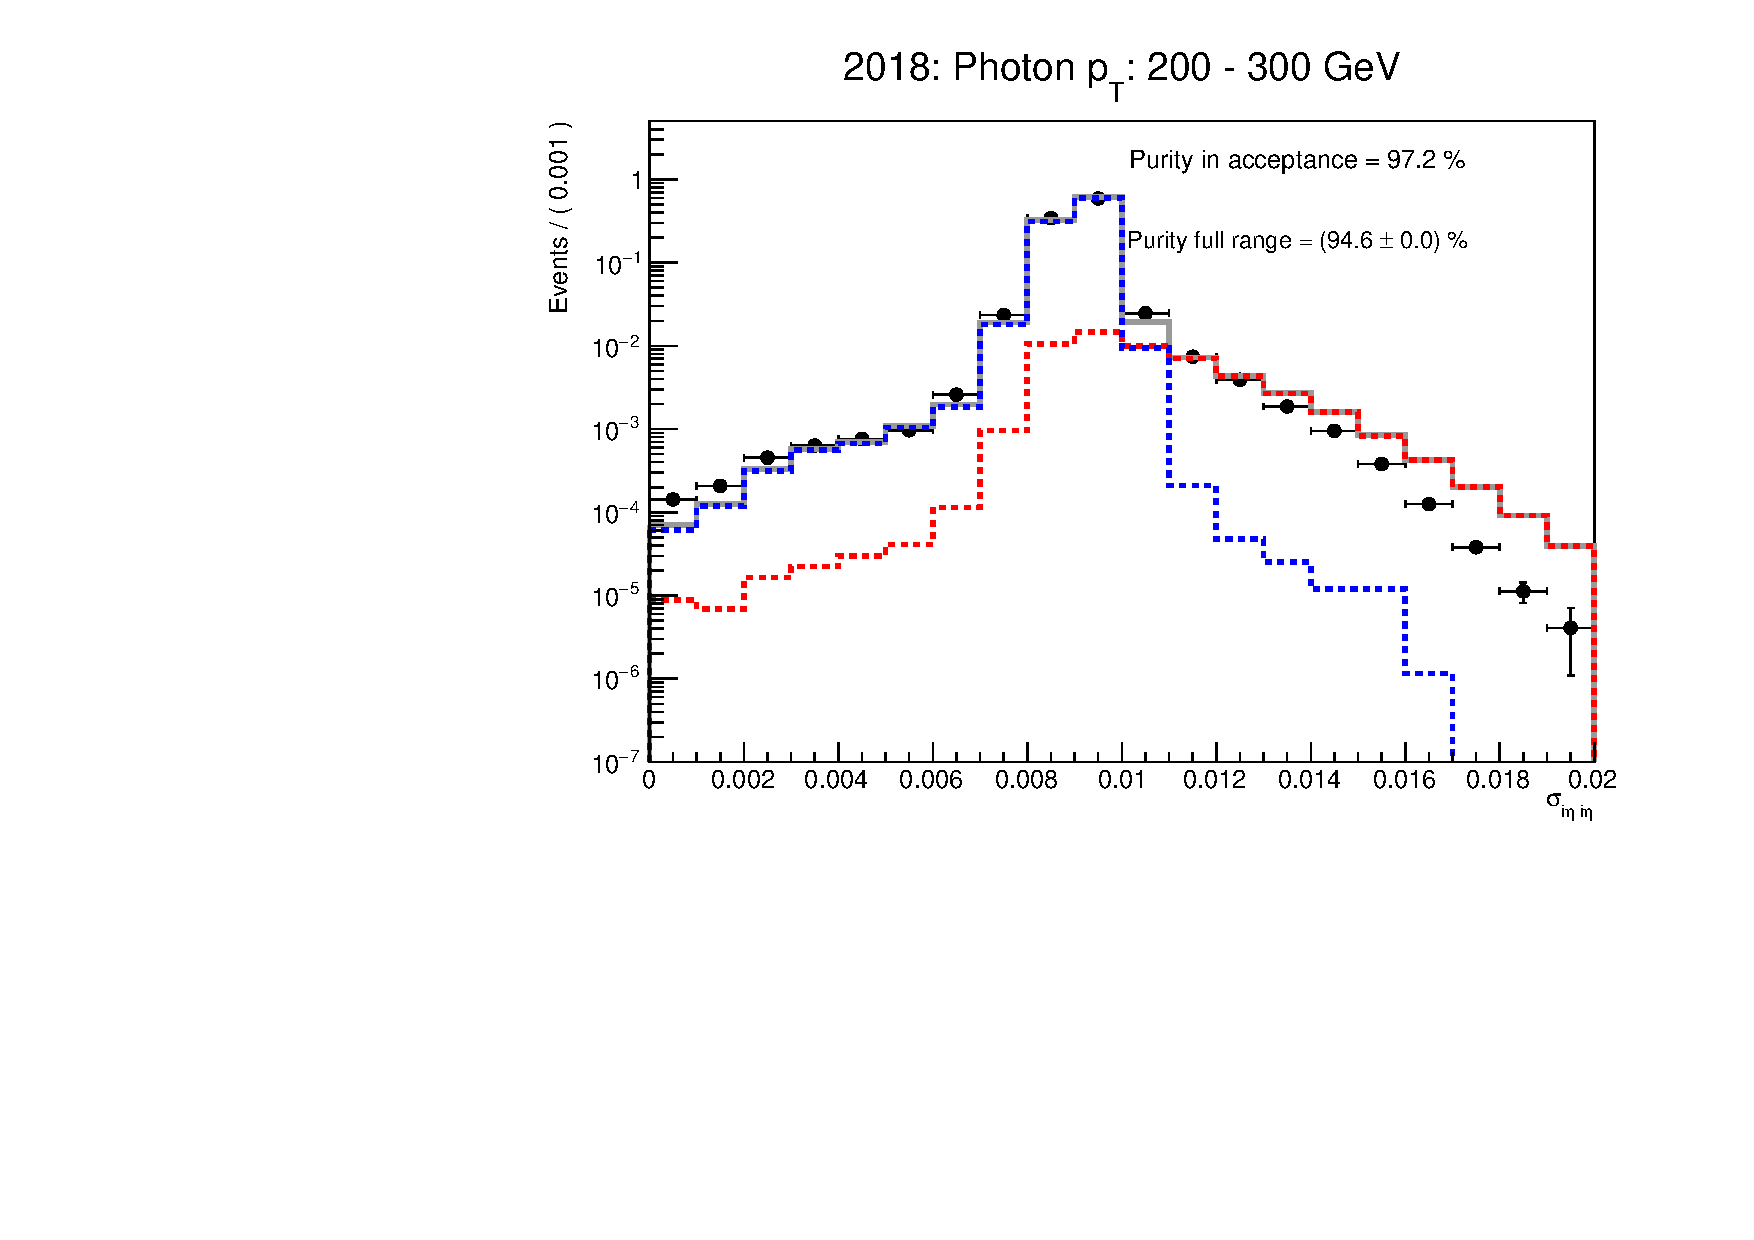
\includegraphics[width=0.45\textwidth]{PhotonPurity/fit_2018_pt200-300_nominal.pdf}
        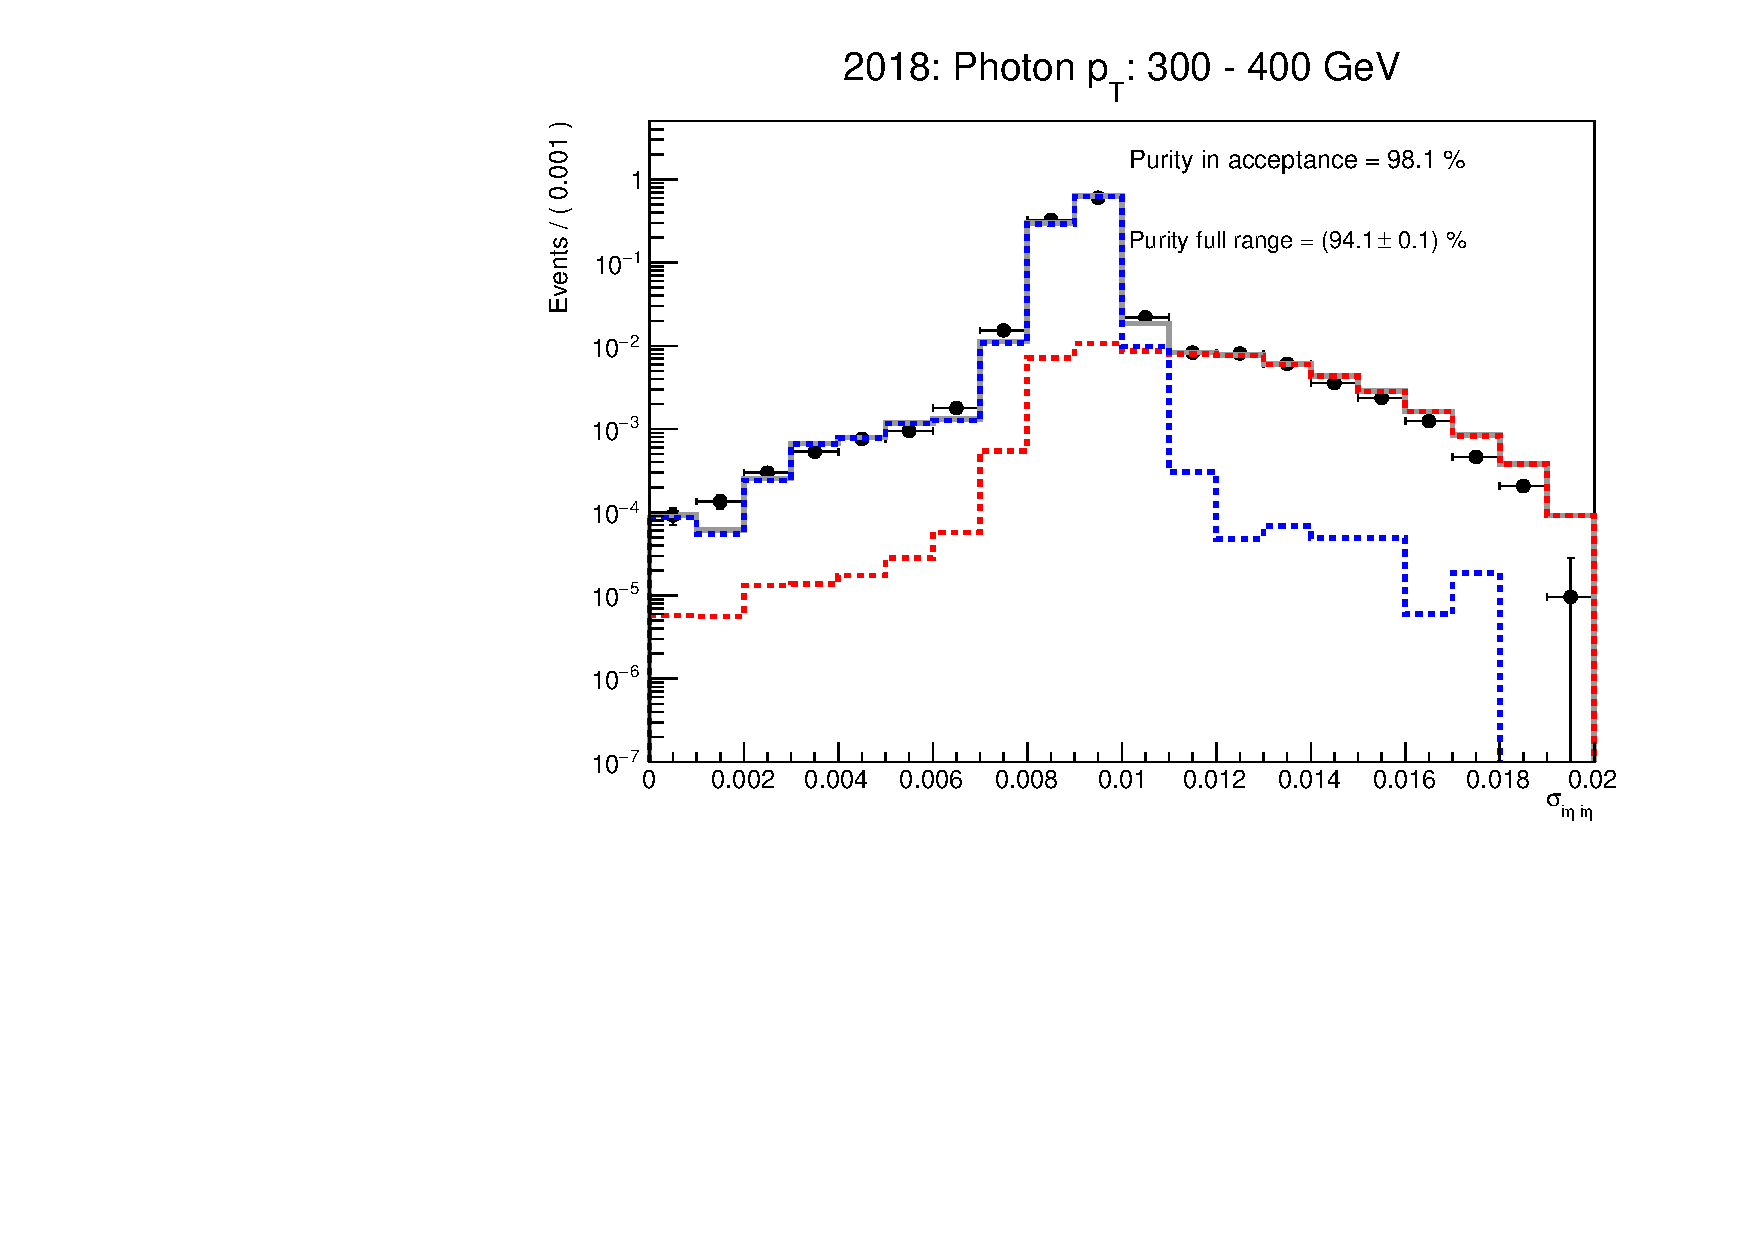
\includegraphics[width=0.45\textwidth]{PhotonPurity/fit_2018_pt300-400_nominal.pdf}
        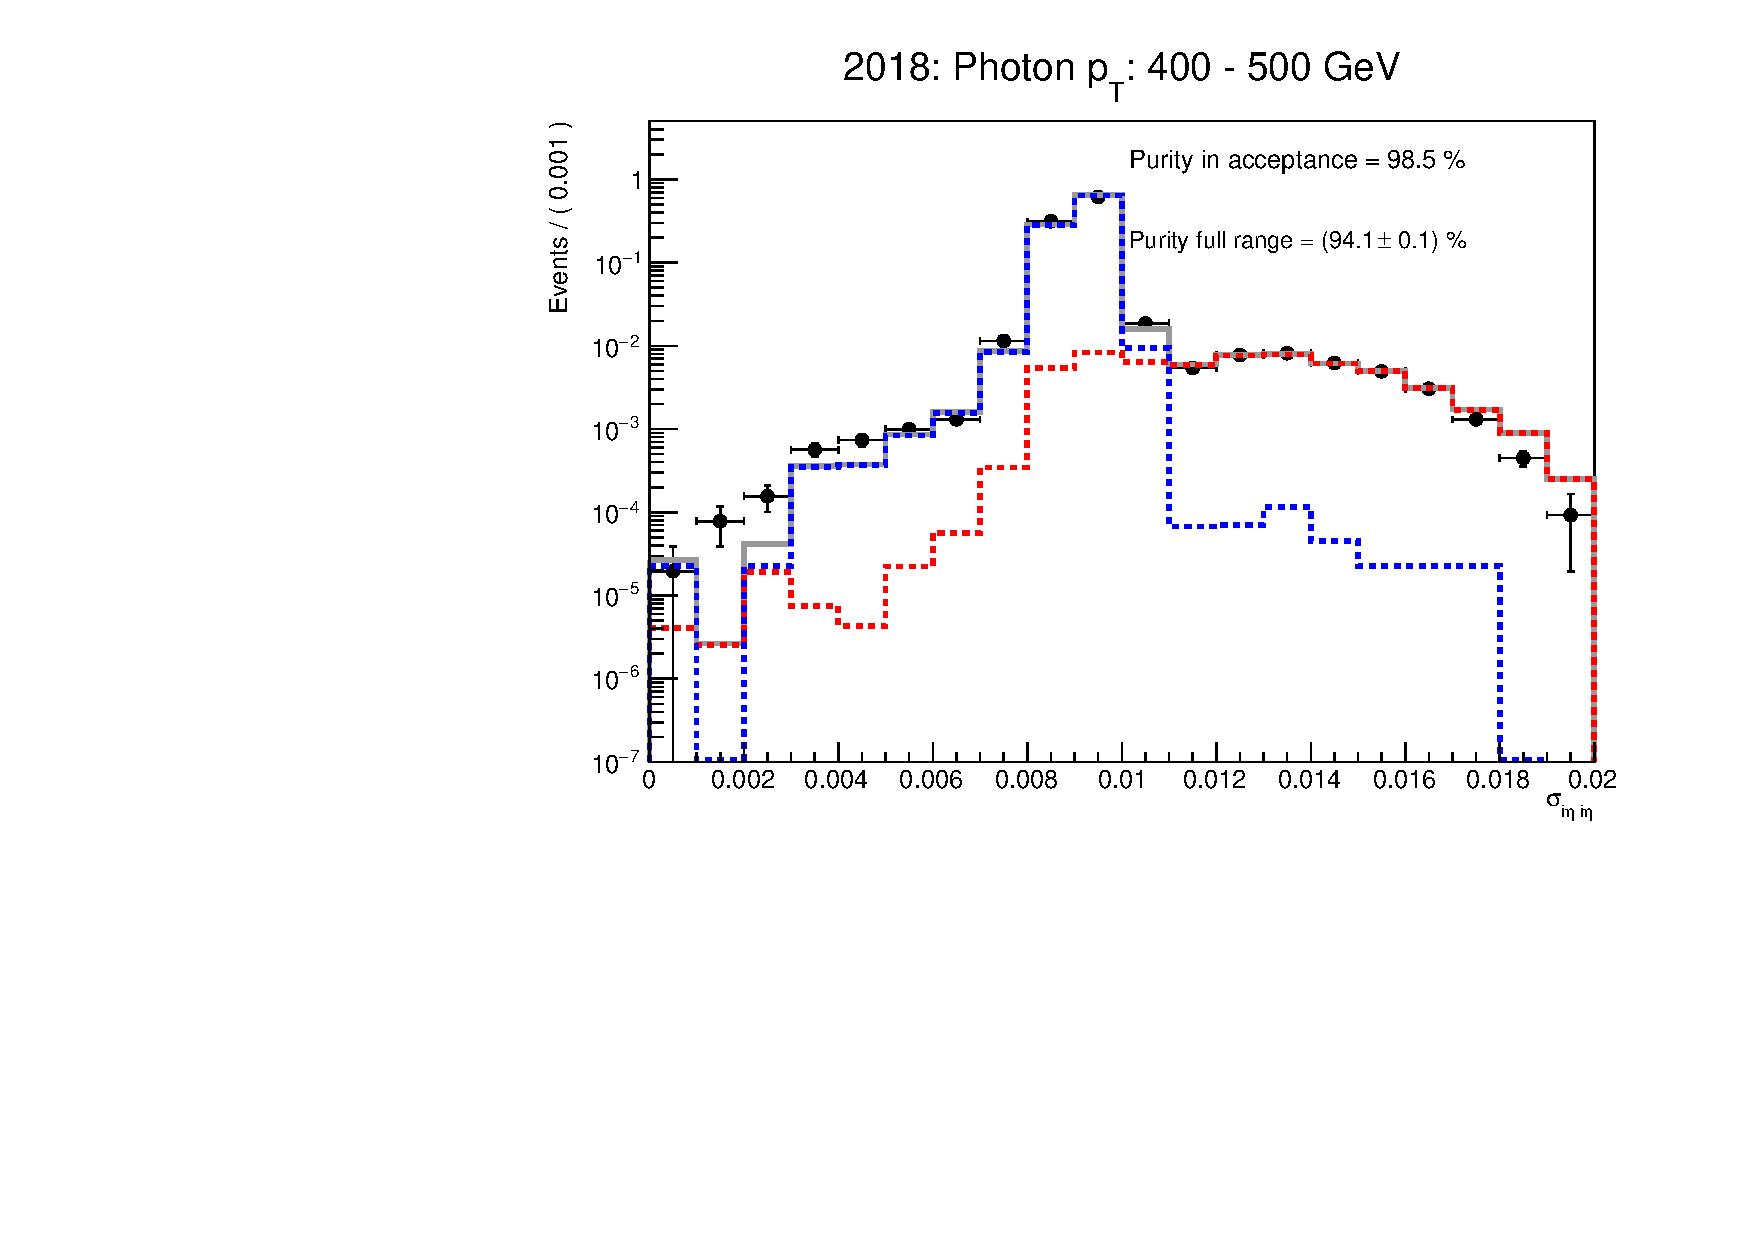
\includegraphics[width=0.45\textwidth]{PhotonPurity/fit_2018_pt400-500_nominal.pdf}
        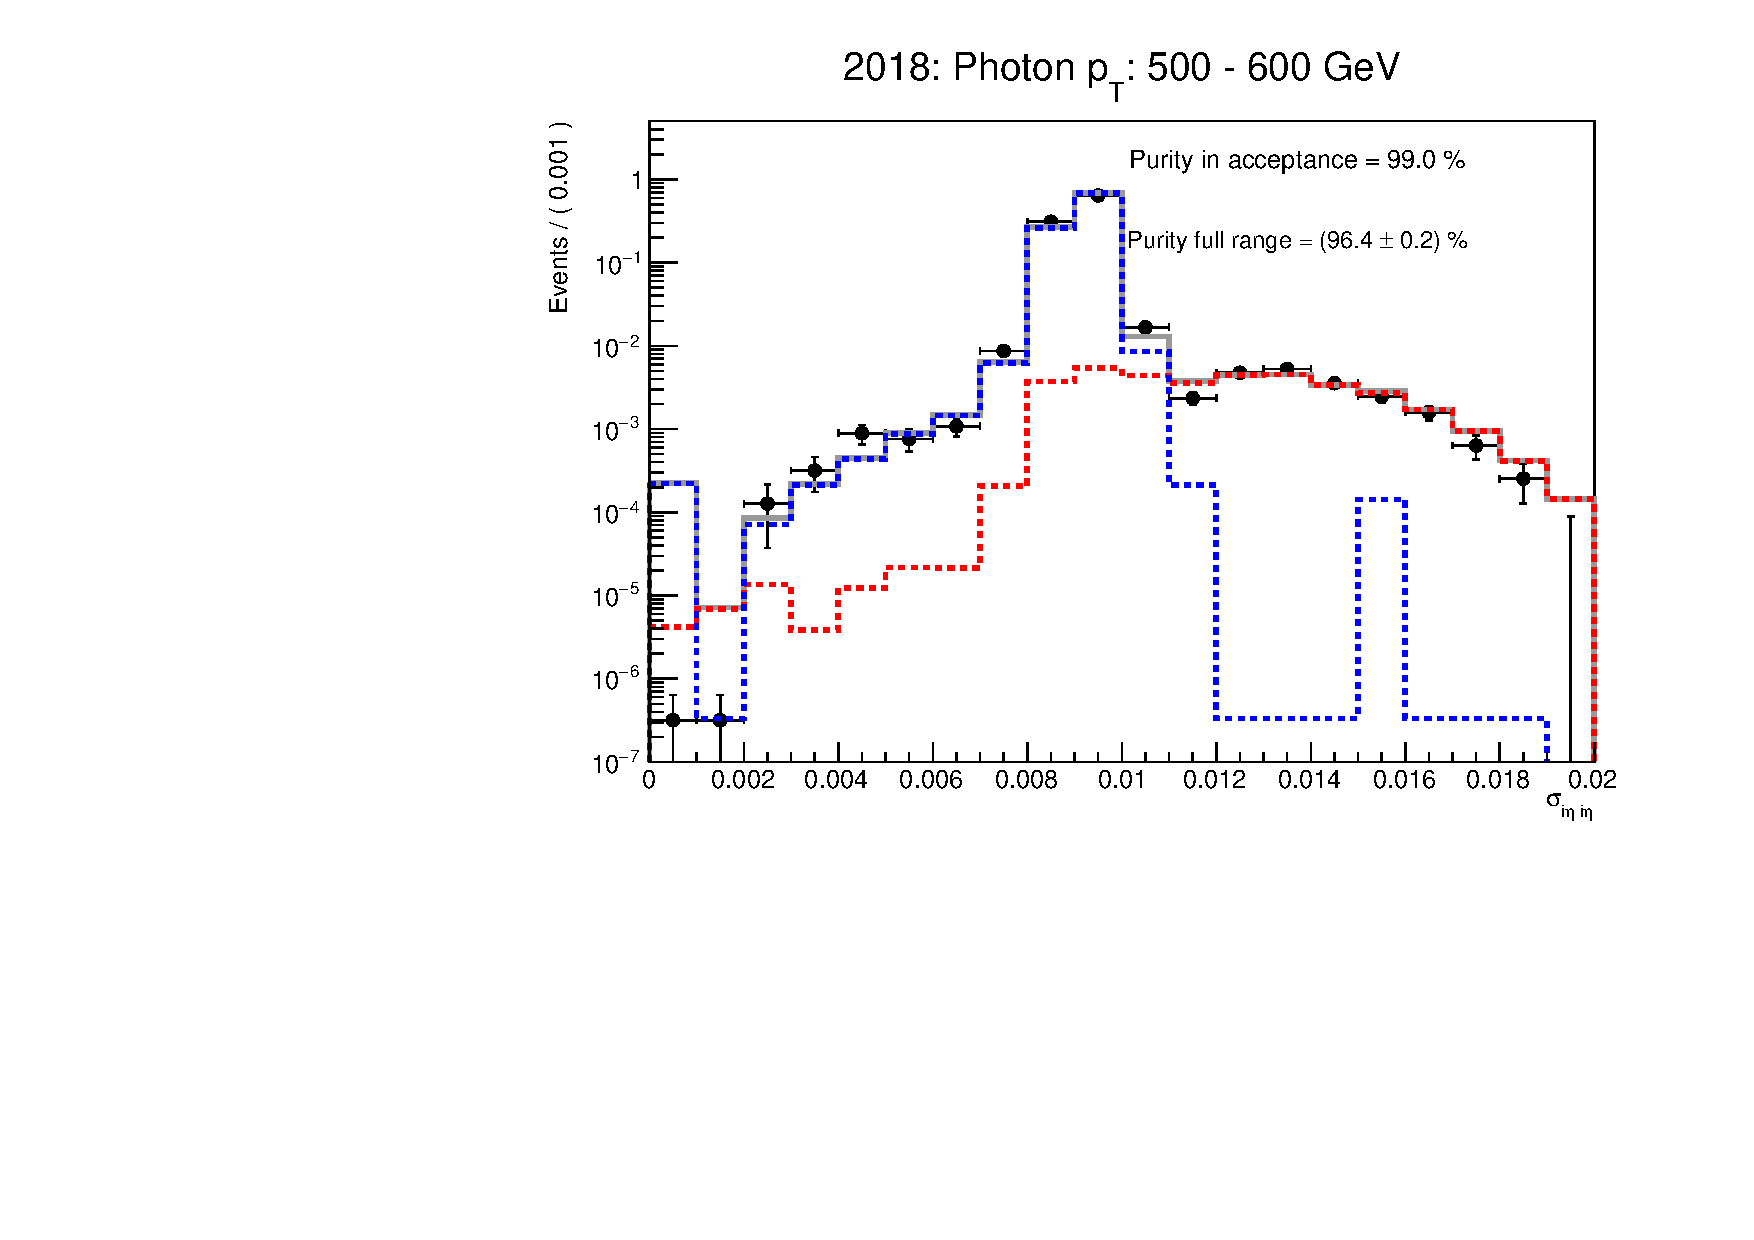
\includegraphics[width=0.45\textwidth]{PhotonPurity/fit_2018_pt500-600_nominal.pdf}
        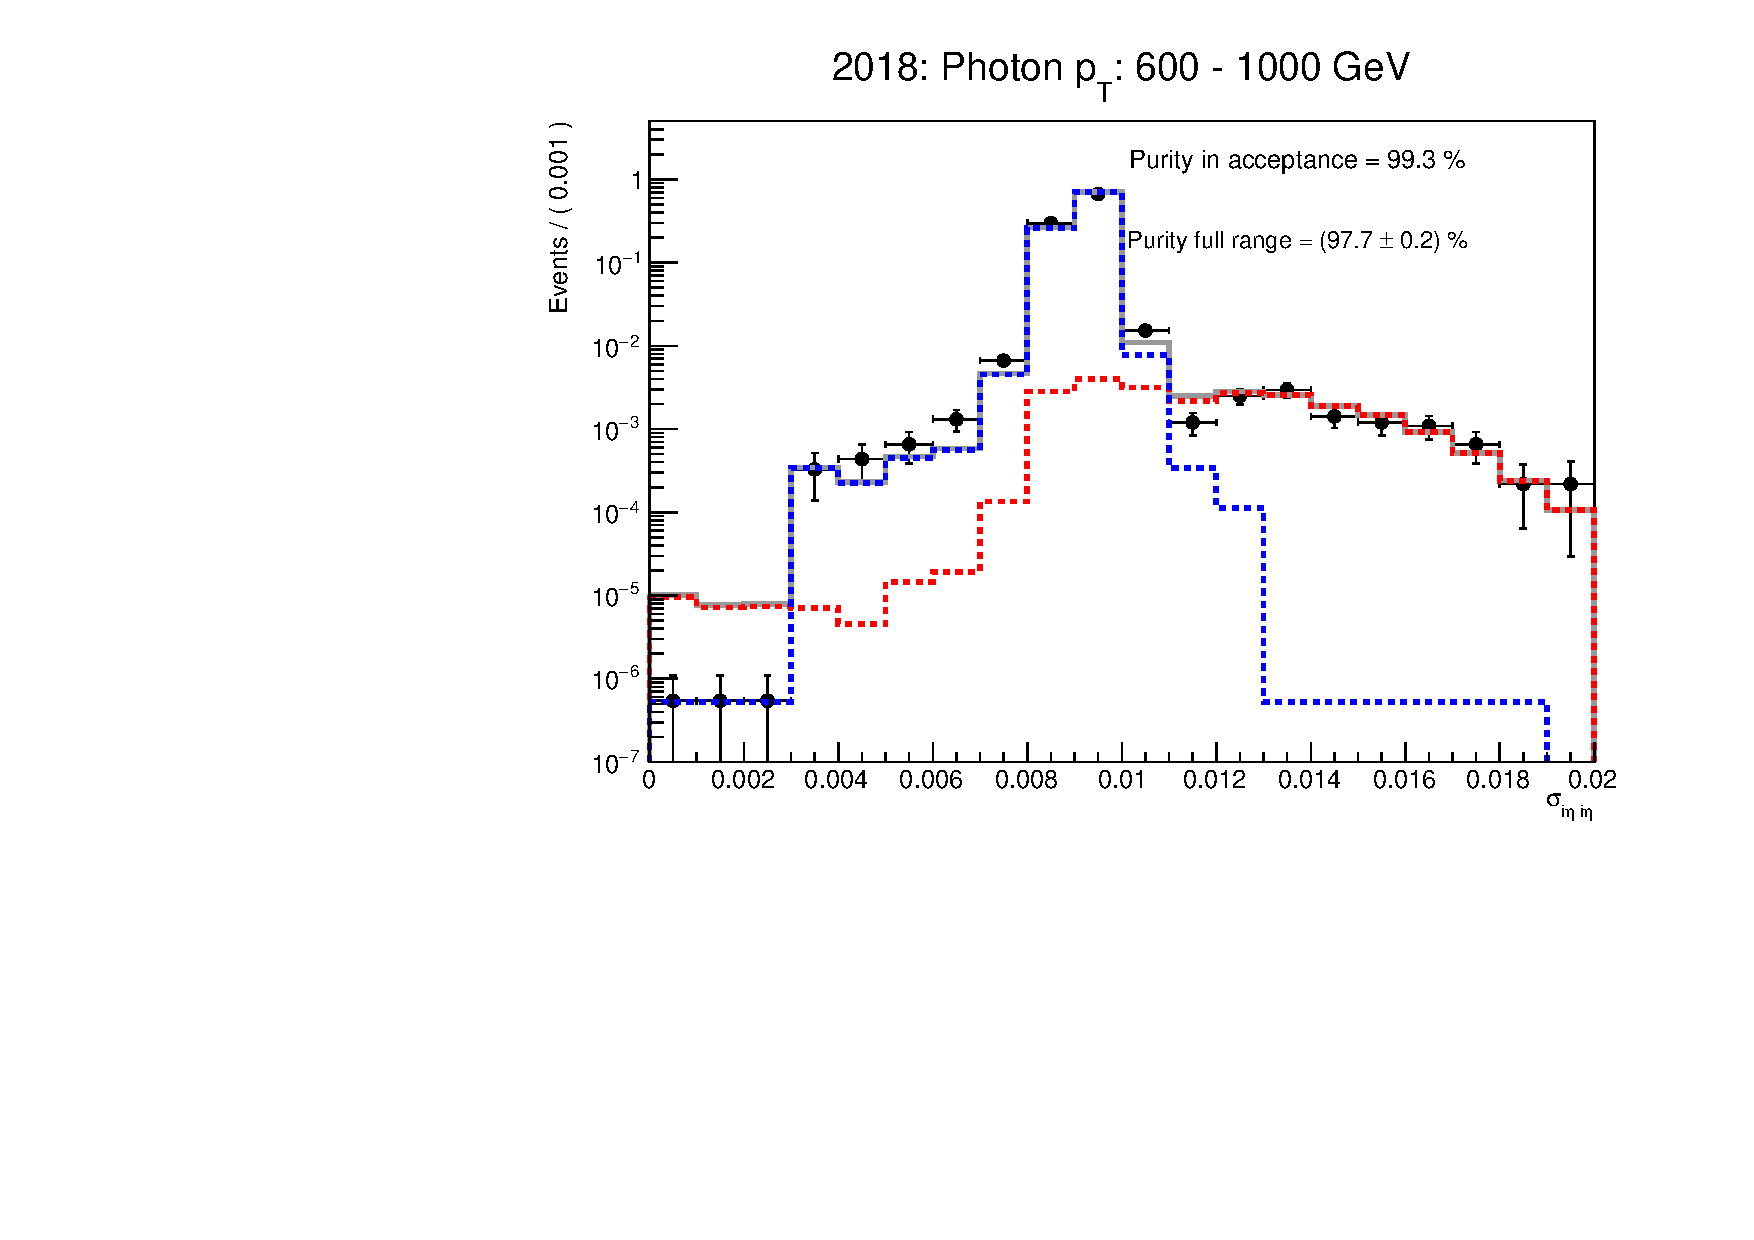
\includegraphics[width=0.45\textwidth]{PhotonPurity/fit_2018_pt600-1000_nominal.pdf}
    \caption{Template fits used to determine the photon purity in the 2018 dataset. The fits are shown in bins of photon \pt, increasing from left 
    to right and top to bottom. The ``nominal'' binning scheme is used.}
    \label{fig:purity_fits_2018}
\end{figure}

\begin{figure}[htbp]
    \centering
        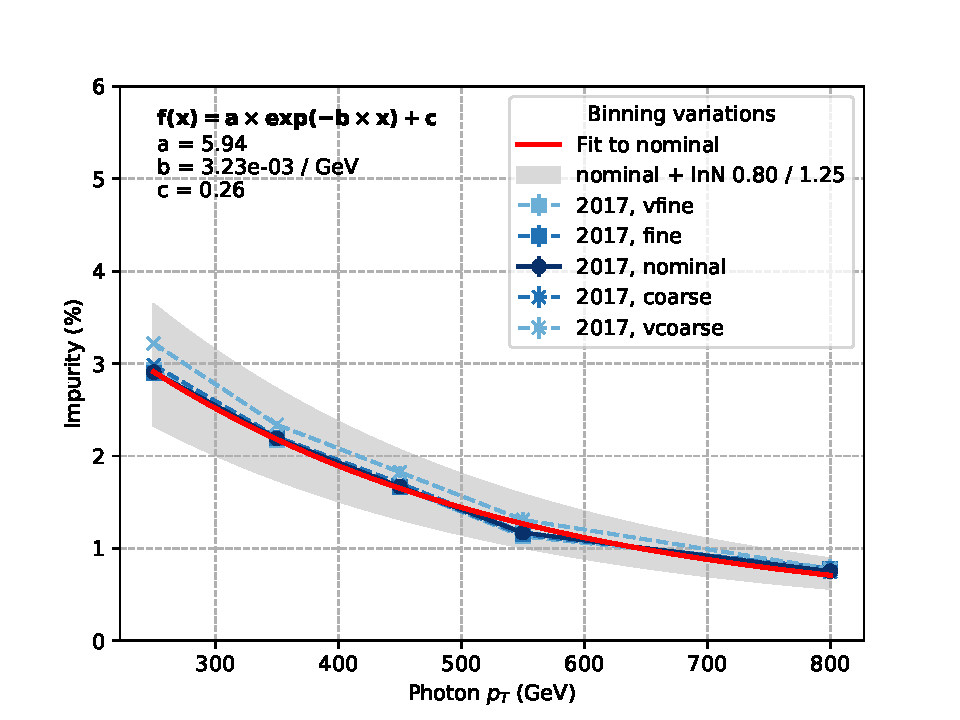
\includegraphics[width=0.48\textwidth]{PhotonPurity/purity_variations_2017.pdf}
        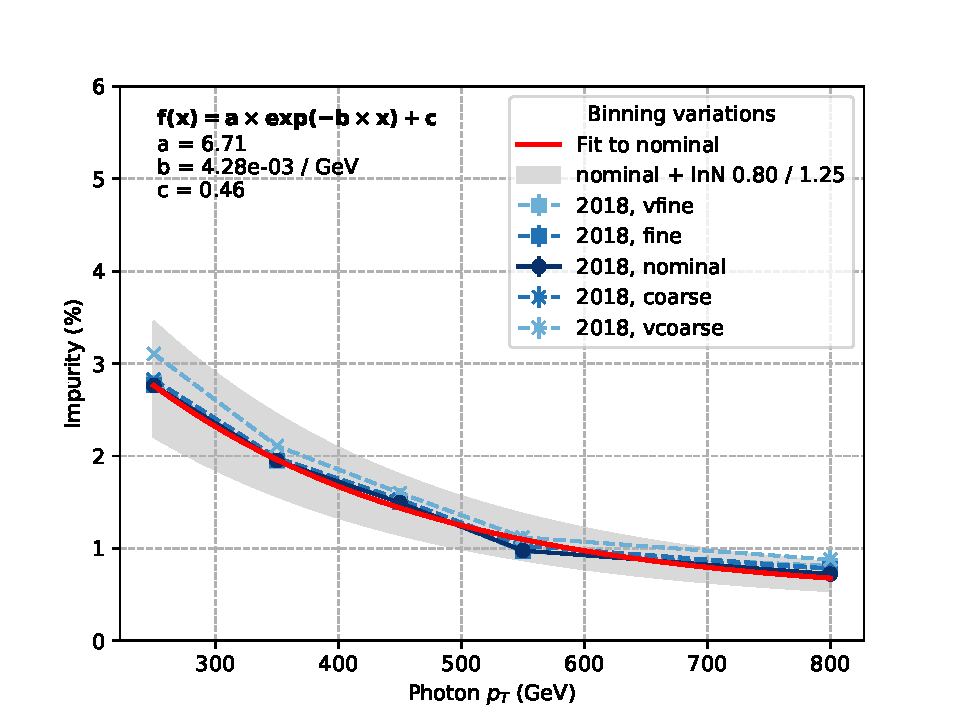
\includegraphics[width=0.48\textwidth]{PhotonPurity/purity_variations_2018.pdf}
    \caption{Photon impurity as a function of photon \pt for 2017 (left) and 2018 (right). The measured values for different binning choices 
    are shown in the blue shaded lines and markers. The nominal result is interpolated using an exponential function fit, which is shown in 
    the red solid line. The gray band represents a 25\% uncertainty around the interpolated nominal result.}
    \label{fig:purity_result}
\end{figure}

\begin{figure}[htbp]
    \centering
        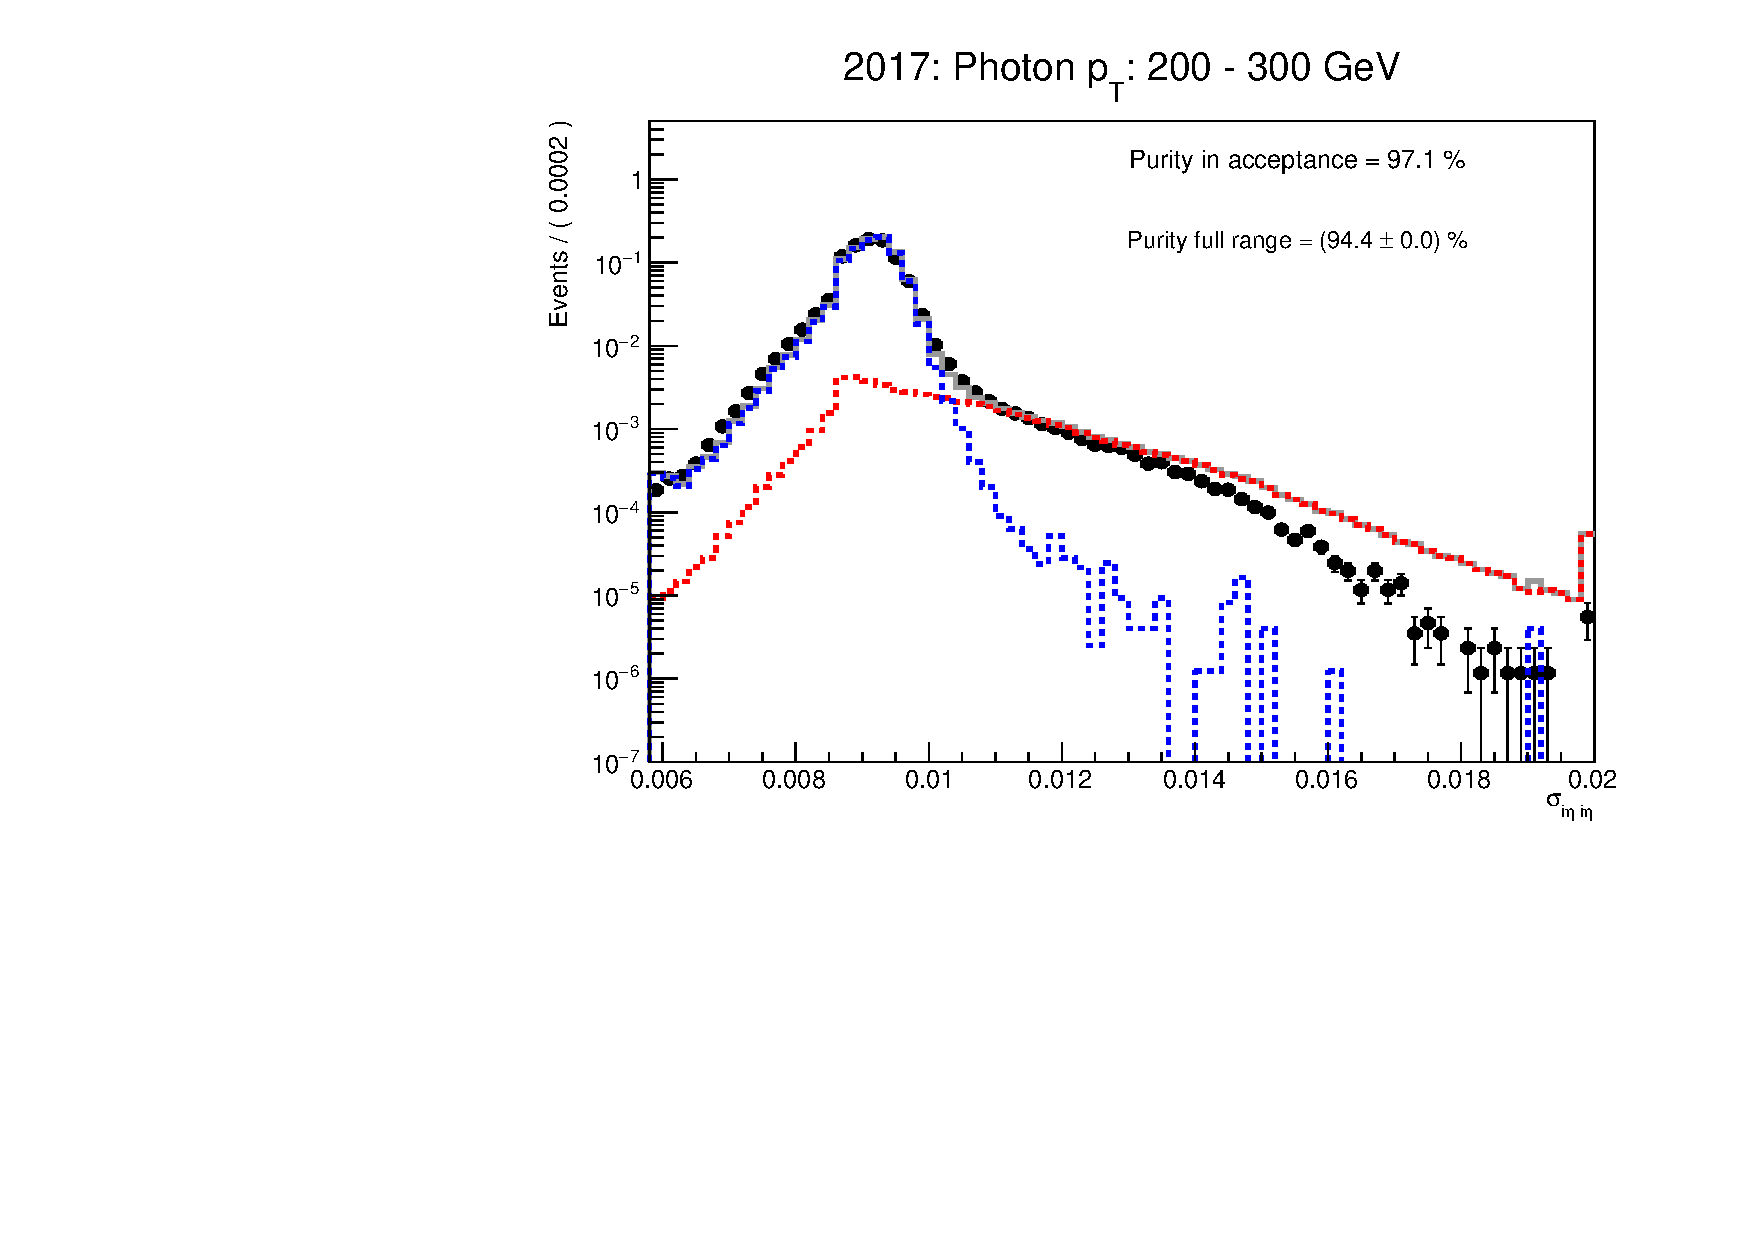
\includegraphics[width=0.45\textwidth]{PhotonPurity/fit_2017_pt200-300_vfine.pdf}
        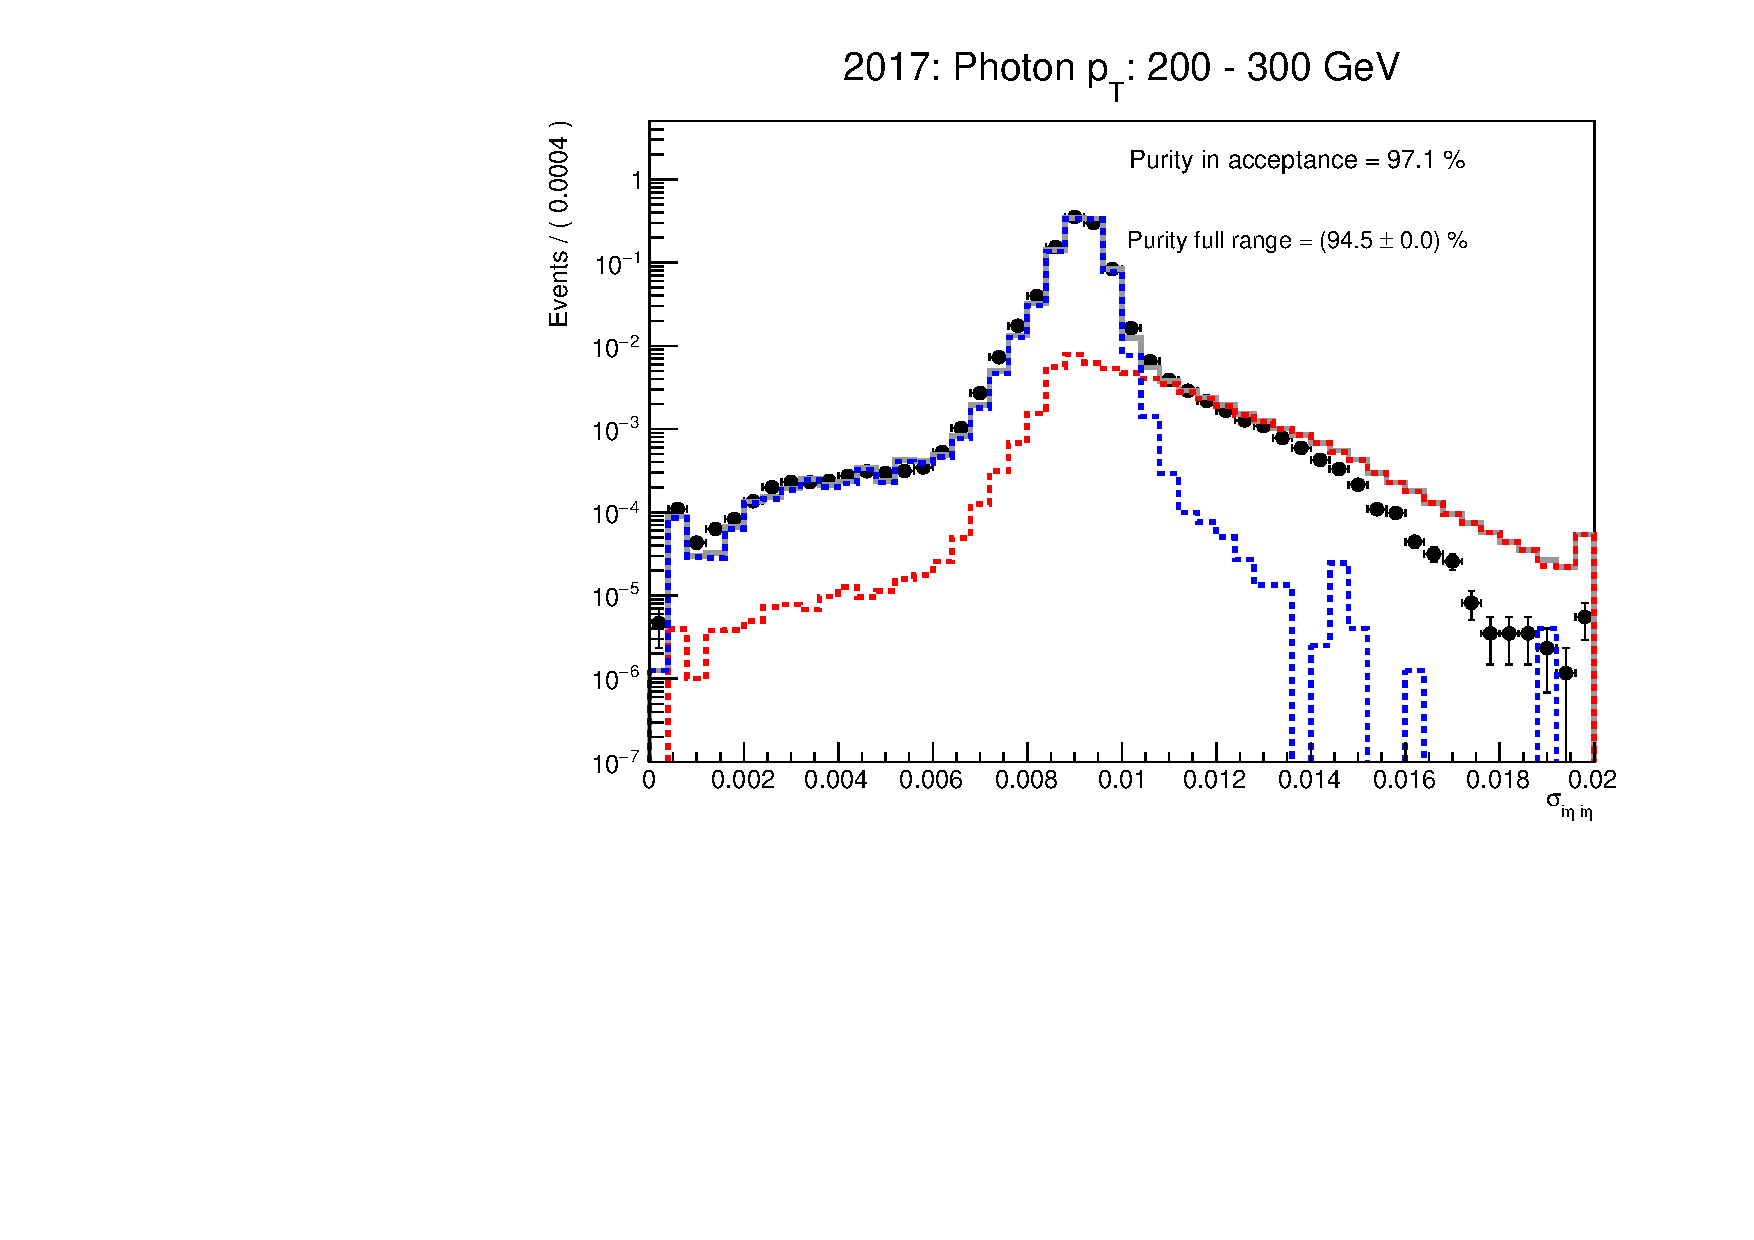
\includegraphics[width=0.45\textwidth]{PhotonPurity/fit_2017_pt200-300_fine.pdf} \\
        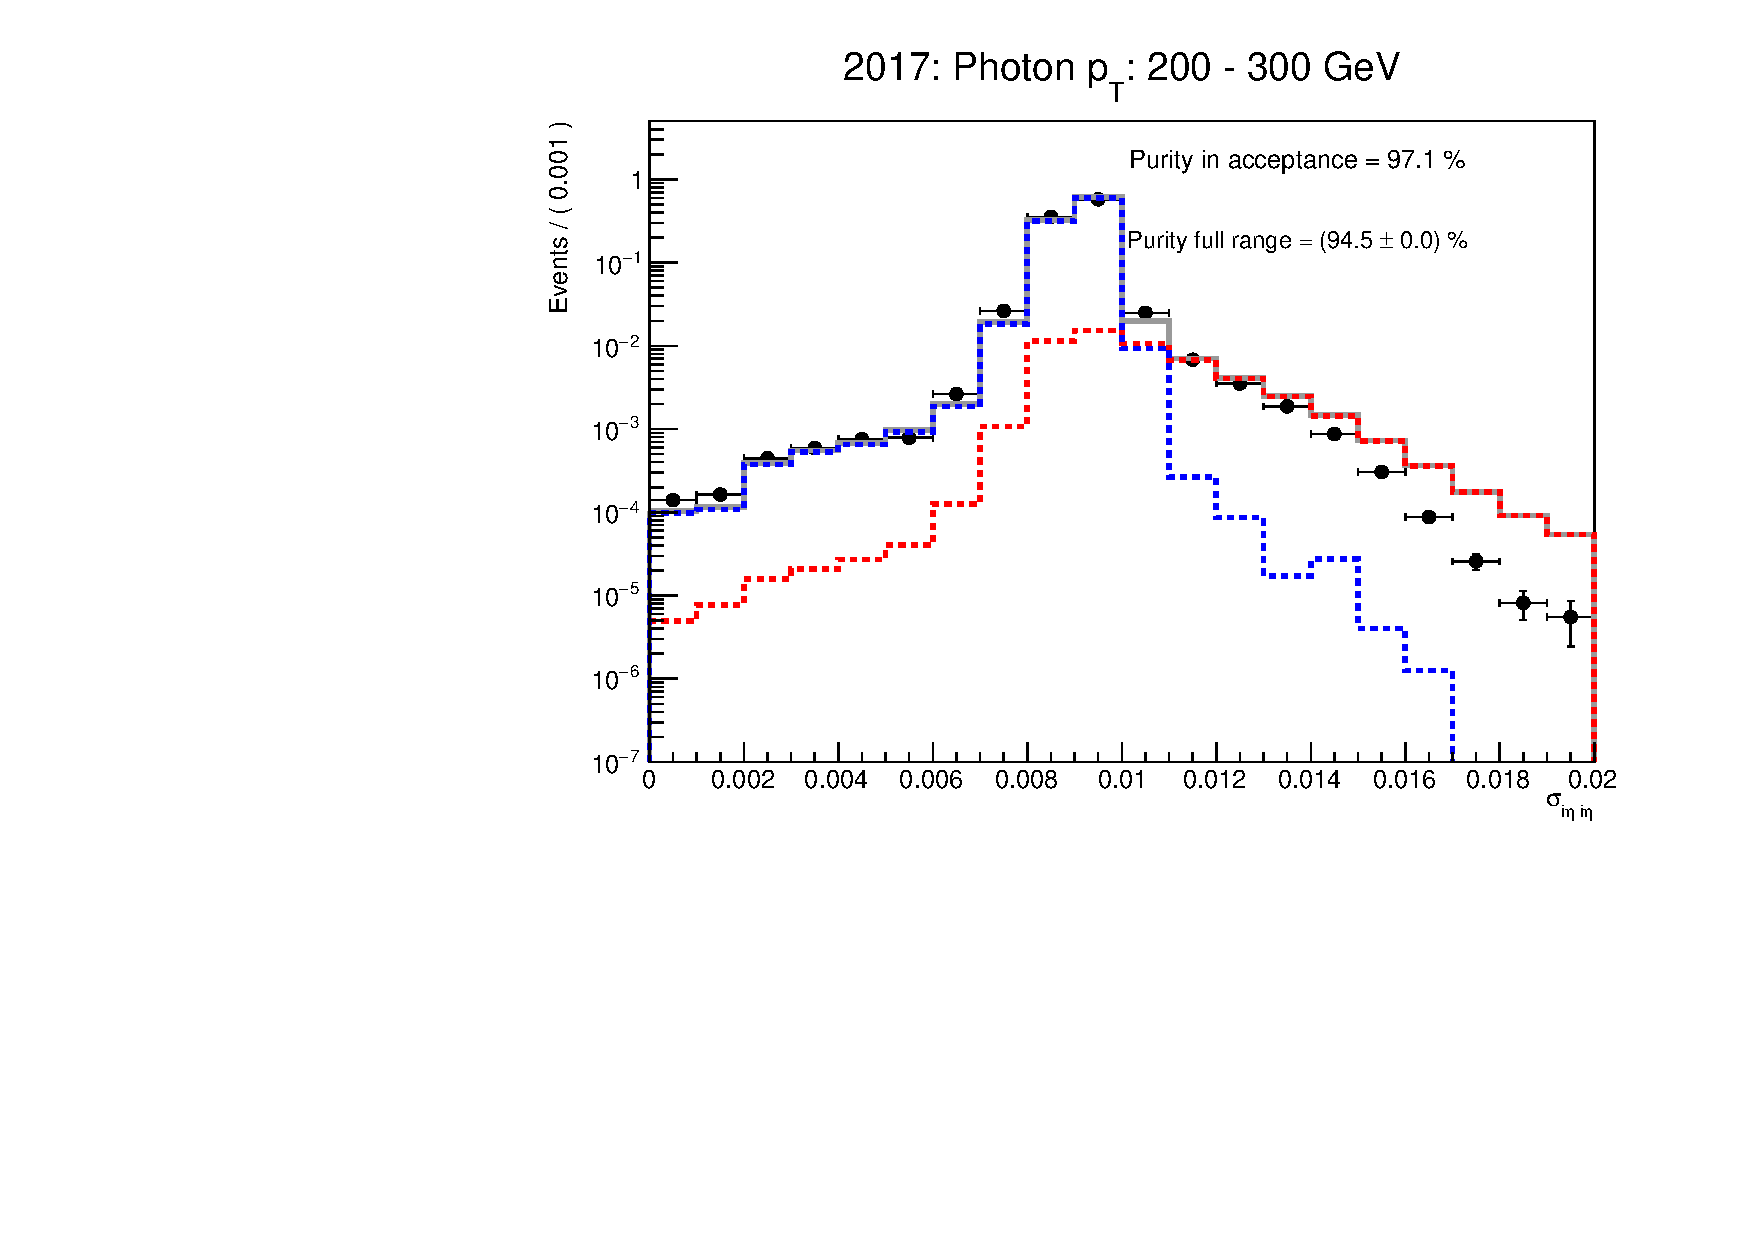
\includegraphics[width=0.45\textwidth]{PhotonPurity/fit_2017_pt200-300_nominal.pdf} \\
        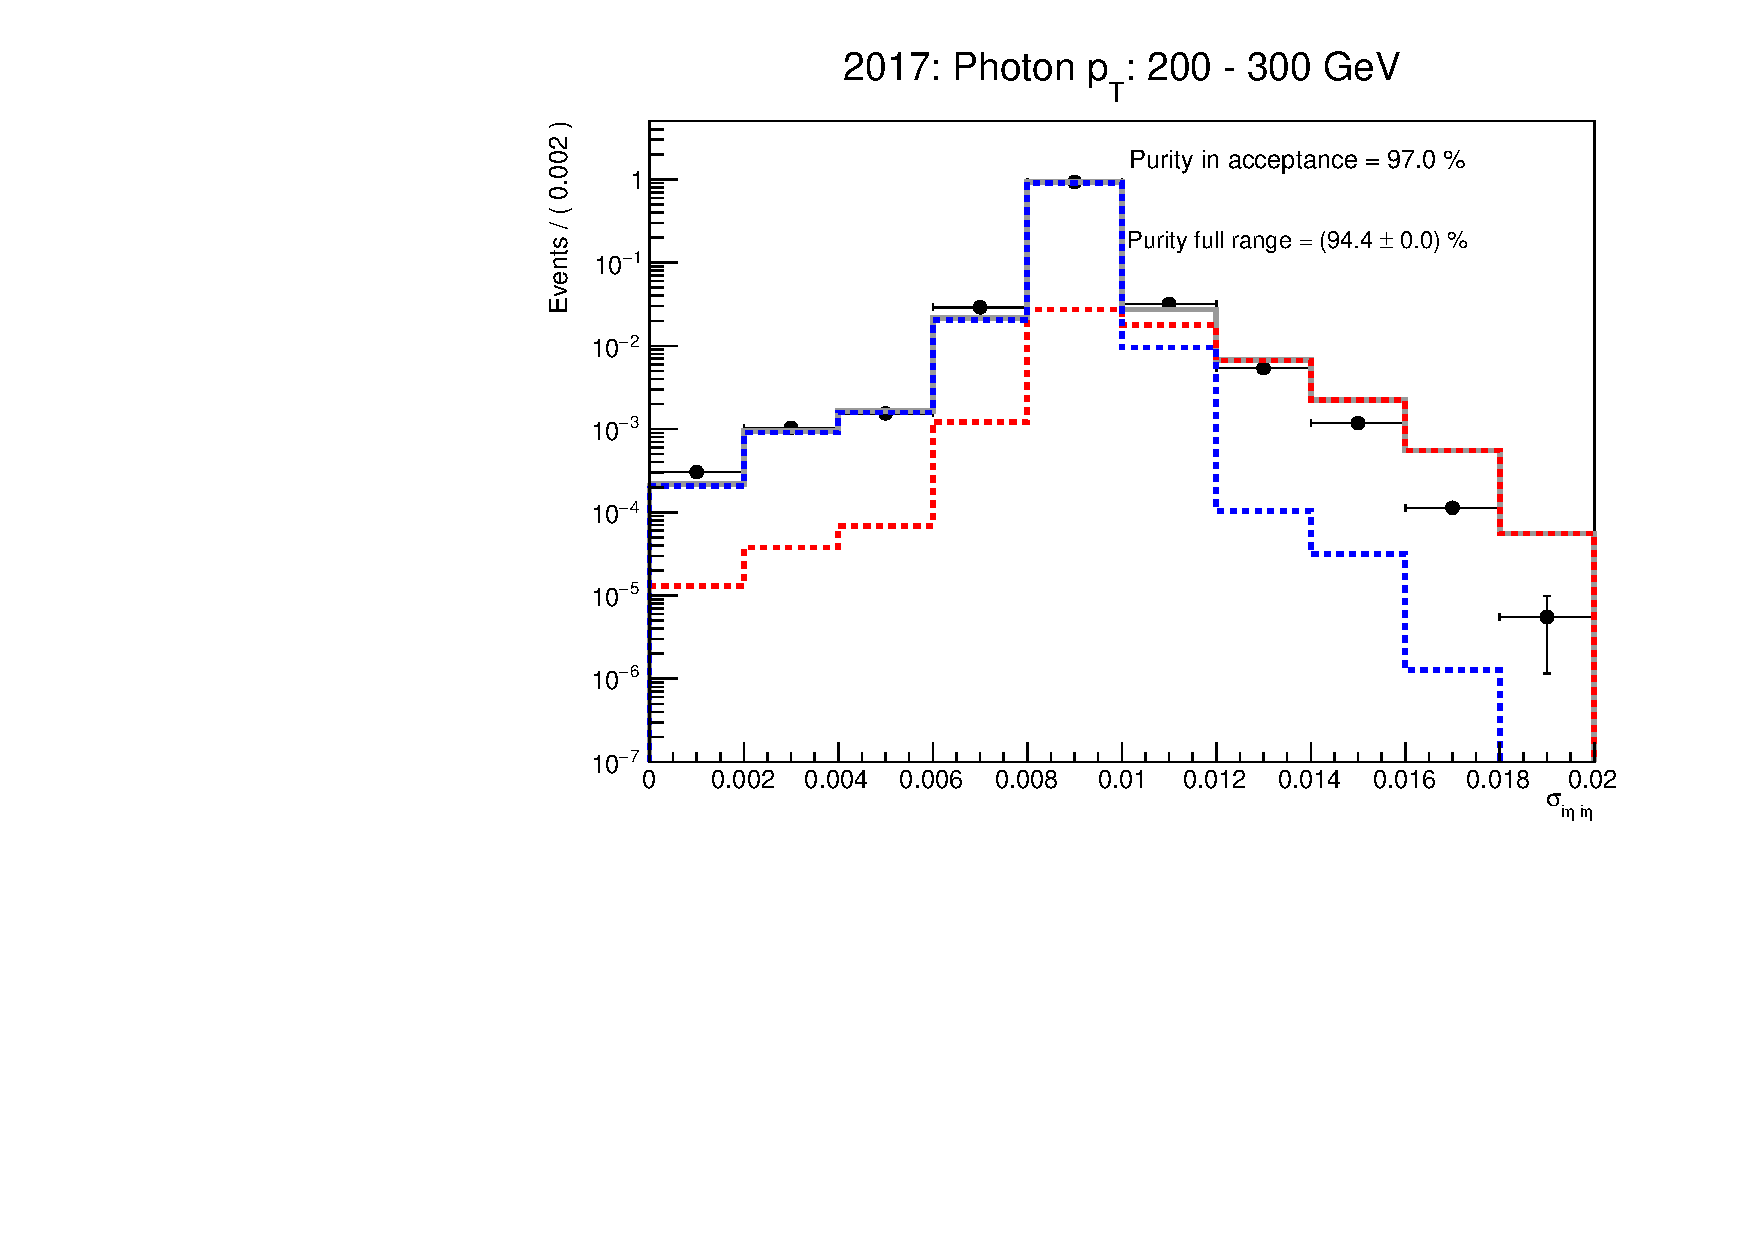
\includegraphics[width=0.45\textwidth]{PhotonPurity/fit_2017_pt200-300_coarse.pdf}
        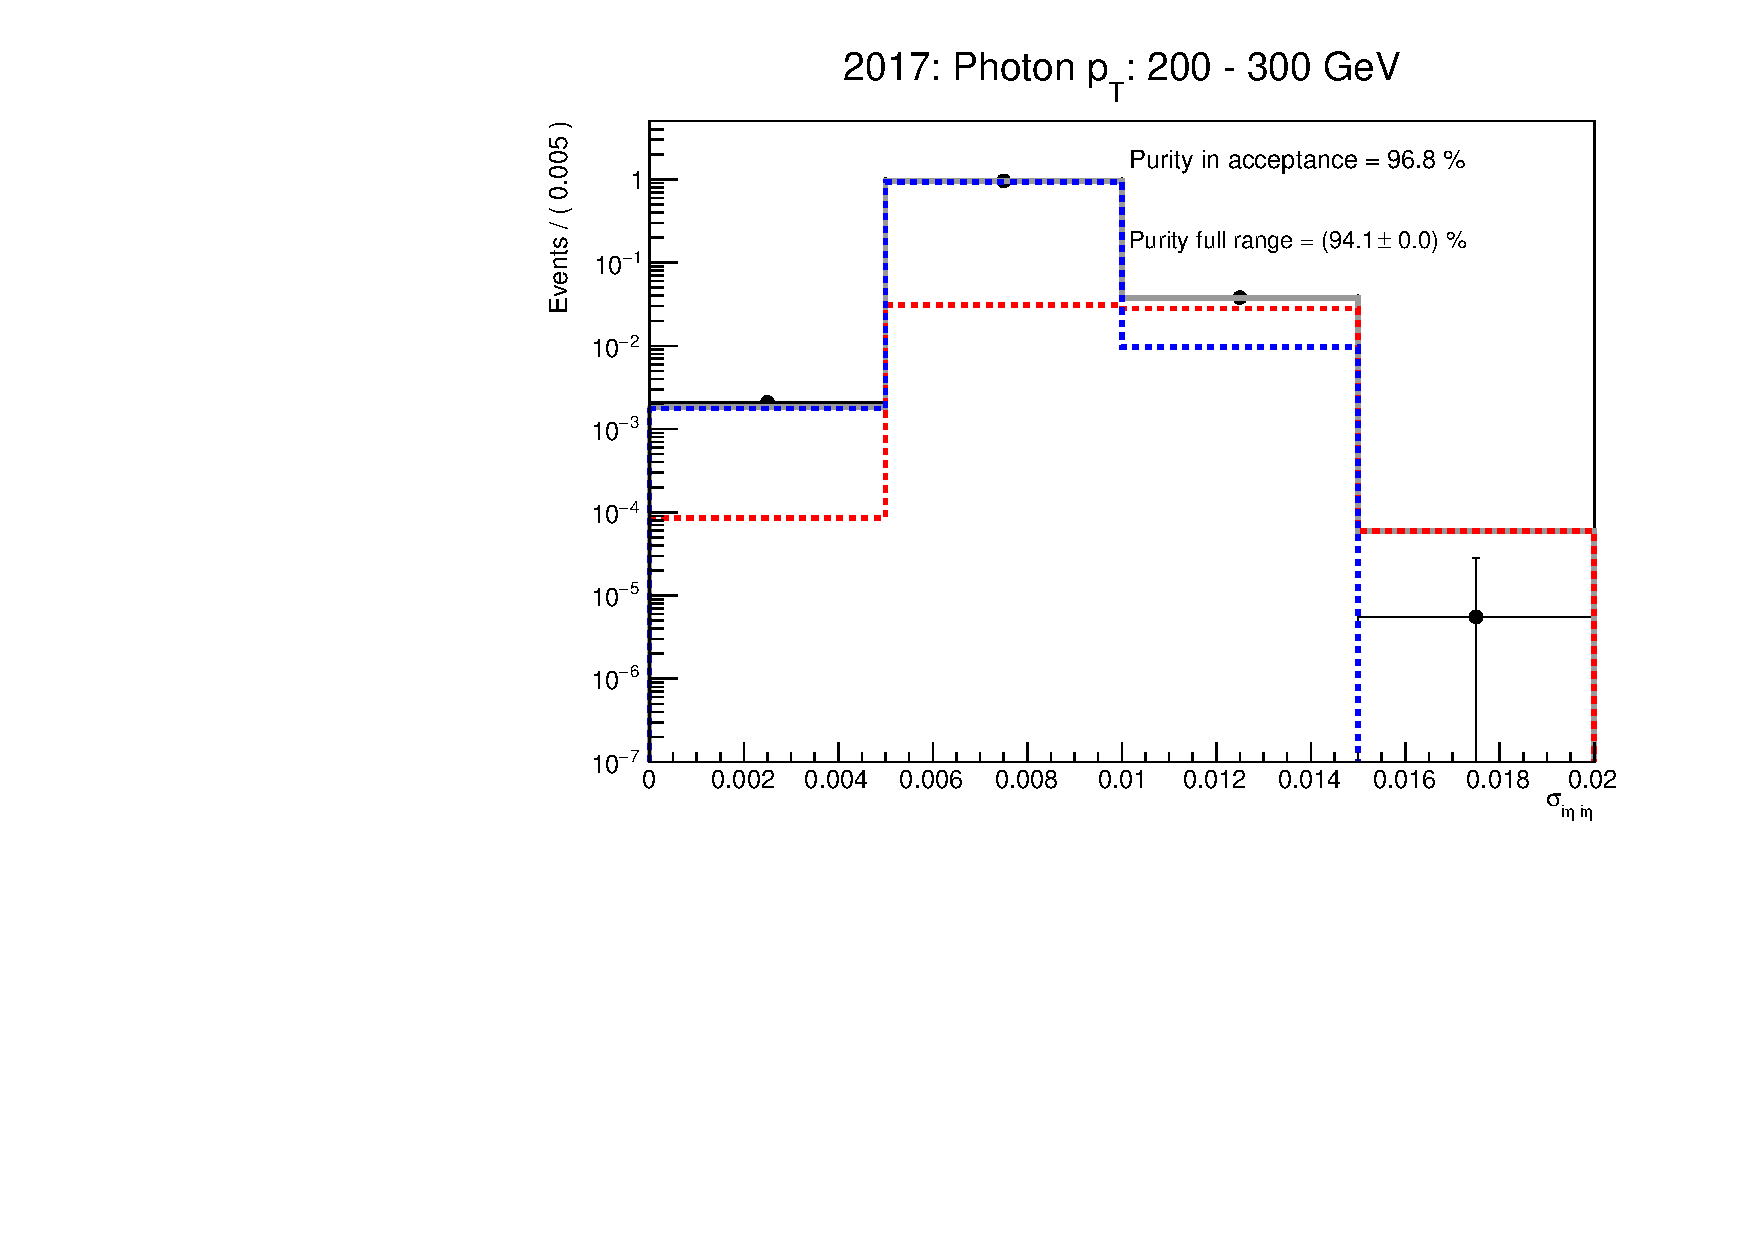
\includegraphics[width=0.45\textwidth]{PhotonPurity/fit_2017_pt200-300_vcoarse.pdf}
    \caption{Comparison of binning schemes used to define a systematic uncertainty on the purity measurement. In all cases, the 
    $200<\pt<300$ GeV bin of the 2017 data set is shown. The binning choices are very fine and fine (top row), nominal (middle row) 
    and coarse and very coarse (bottom row).}
    \label{fig:purity_binning}
\end{figure}

\clearpage